\documentclass[10pt,letterpaper]{article}
\usepackage{geometry}
\geometry{margin=1in}
\usepackage{graphicx}
\graphicspath{{../figs/}{figs/}}
\usepackage{subcaption}
\usepackage{wrapfig}
\usepackage{float}
\setlength{\parindent}{0pt}
\setlength{\parskip}{0.5em}
\usepackage{multirow}
%make lists tighter
\usepackage{enumitem}
\usepackage{booktabs}
\setlist{nolistsep}
\usepackage{subcaption} 

%reduce spacing before and after section
\usepackage{titlesec}
% reduce section, subsection, etc spacing
\usepackage{titlesec}
\titlespacing*{\section}{0pt}{0\baselineskip}{0\baselineskip}
\titlespacing*{\subsection}{0pt}{0\baselineskip}{0\baselineskip}
\titlespacing*{\subsubsection}{0pt}{0\baselineskip}{0\baselineskip}

%reduce list spacing
\usepackage{enumitem}
\setlist{nosep}
\bibliographystyle{plain}   % or unsrt / alpha / apalike
\usepackage[hidelinks]{hyperref}

%improve table visualization
\usepackage{amsmath}
\usepackage{makecell}
\usepackage{booktabs}
\usepackage{tabularx}
\usepackage{array}


\title{Lab 2 - Cloud Data, Stat 214, Spring 2026\vspace{-2em}}

% submission must not contain any of your names
% but feel free to make a version for yourself with your names on it
% \author{Your names}

\begin{document}
\maketitle

% Please use this structure for your report. Your report should be no more than 20 pages, including figures, but excluding bibliography and academic honesty. Do not include \emph{any} code or code output in your report. 

\section{Introduction}

Carbon dioxide intensifies the natural greenhouse effect that occurs within Earth’s atmosphere. Increased temperatures in the Arctic results in changes to the properties and distribution of its ice and snow covered surfaces. These changes lead to continued warming and strong sensitivity to atmospheric carbon. Clouds have a significant influence on the sensitivity of the Arctic's climate. Discerning the properties of clouds in the Arctic is a difficult task, because of the confounding effects of water in other states of matter (ice and snow covered surfaces). Accurate characterization of clouds is necessary to assess the true impact of clouds on future warming in the Arctic. Here we evaluate features captured through the Multiangle Imaging SpectroRadiometer (MISR) that exists on the NASA Terra satellite. Electromagnetic radiation measurements are taken at nine different view angles. We aim to reveal meaningful patterns of image data that help to discern meaningful cloud properties over daylight Arctic through statistical methods. 

\section{EDA}

\subsection{First Glimpse}

On our first review of the expert labeled image data, the presence and absence of clouds is seemingly outlined by unlabeled points. Only pixels that the expert was highly confident of were labeled, meaning expert labels are conservatively given. This indicates the regions where clouds end can be overcome with noise. Figure~\ref{fig:three_labeled_images} outlines this difficulty, particularly with image O012791 which only had 47\% of the pixels labeled. 
\begin{figure}[h]
    \centering

    \begin{subfigure}{0.3\linewidth}
        \centering
        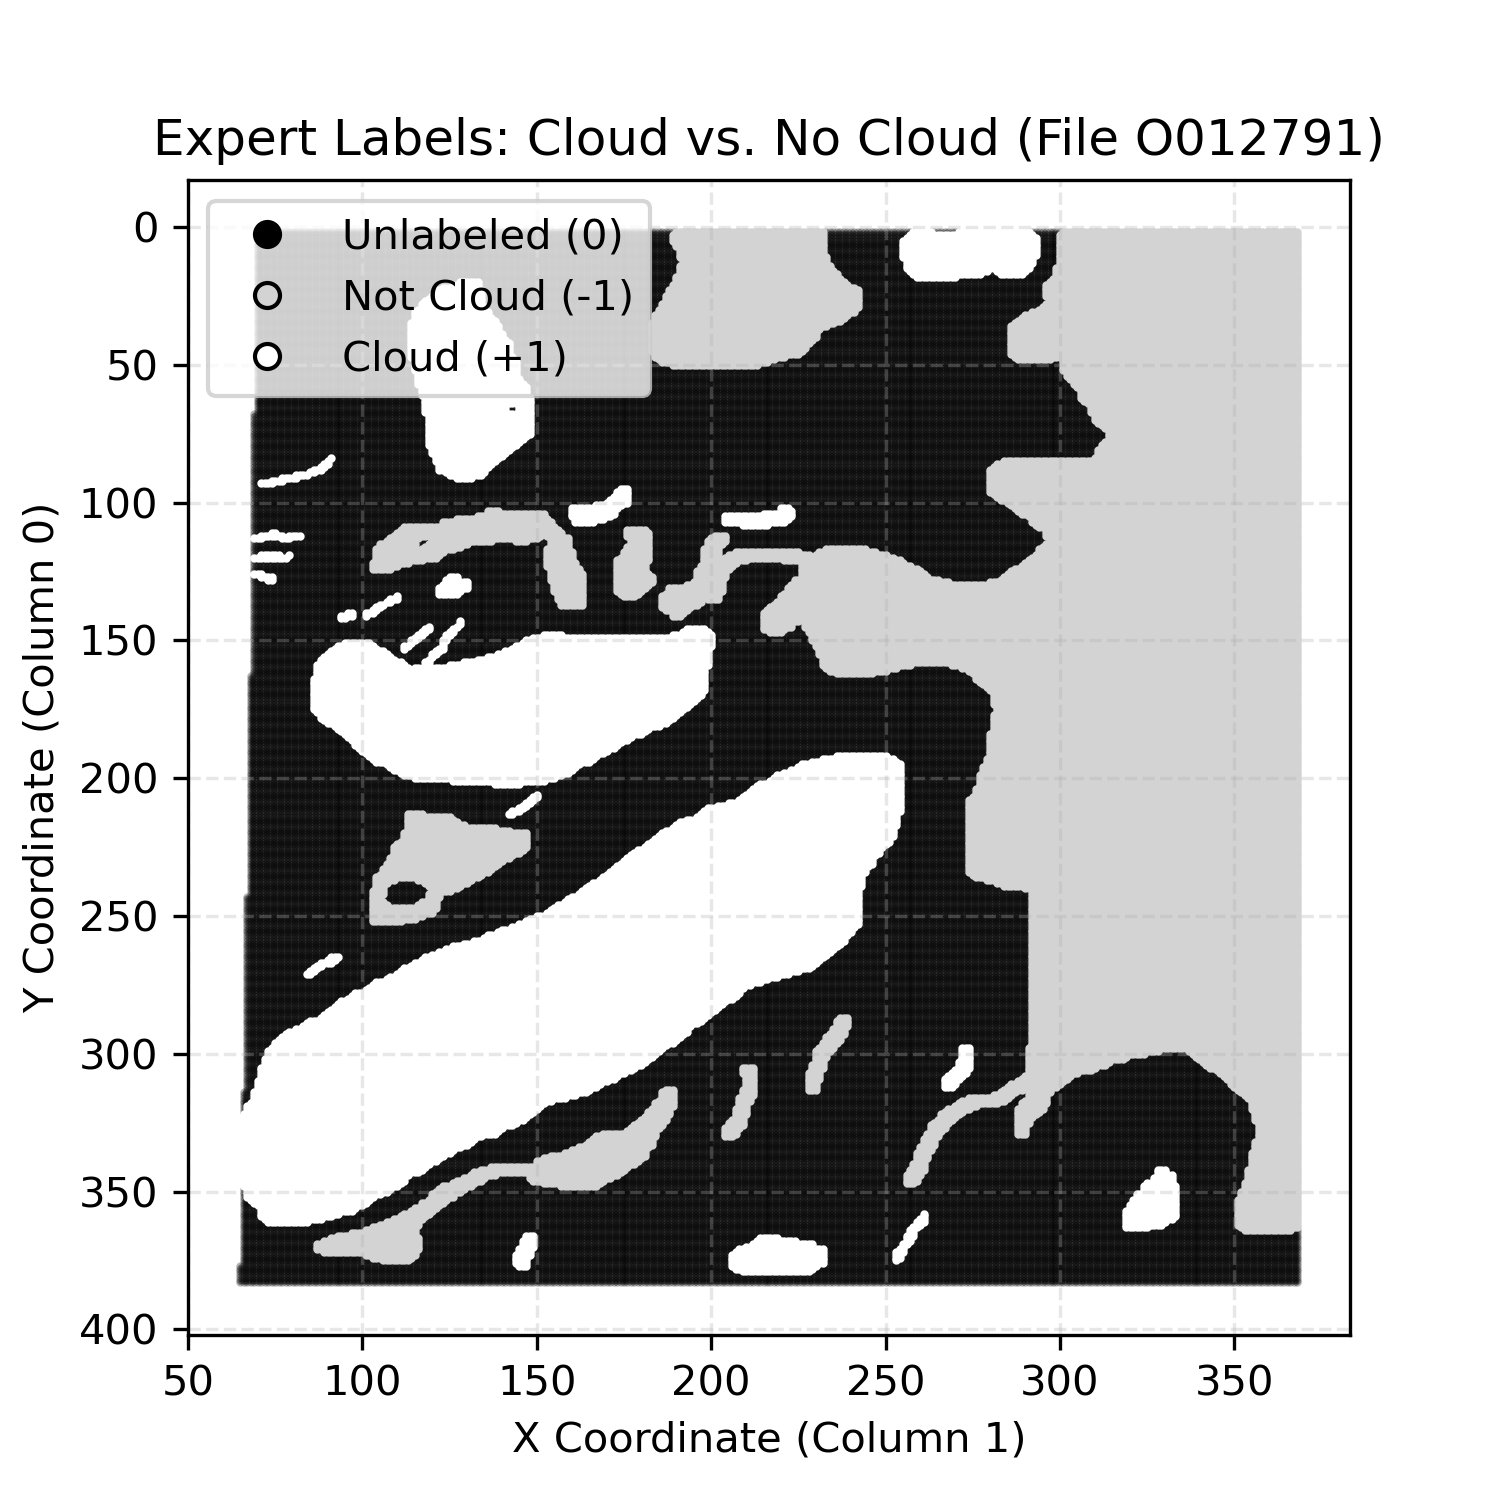
\includegraphics[width=\linewidth]{../figs/O012791.png}
        \caption{Image O012791}
    \end{subfigure}
    \hfill
    \begin{subfigure}{0.3\linewidth}
        \centering
        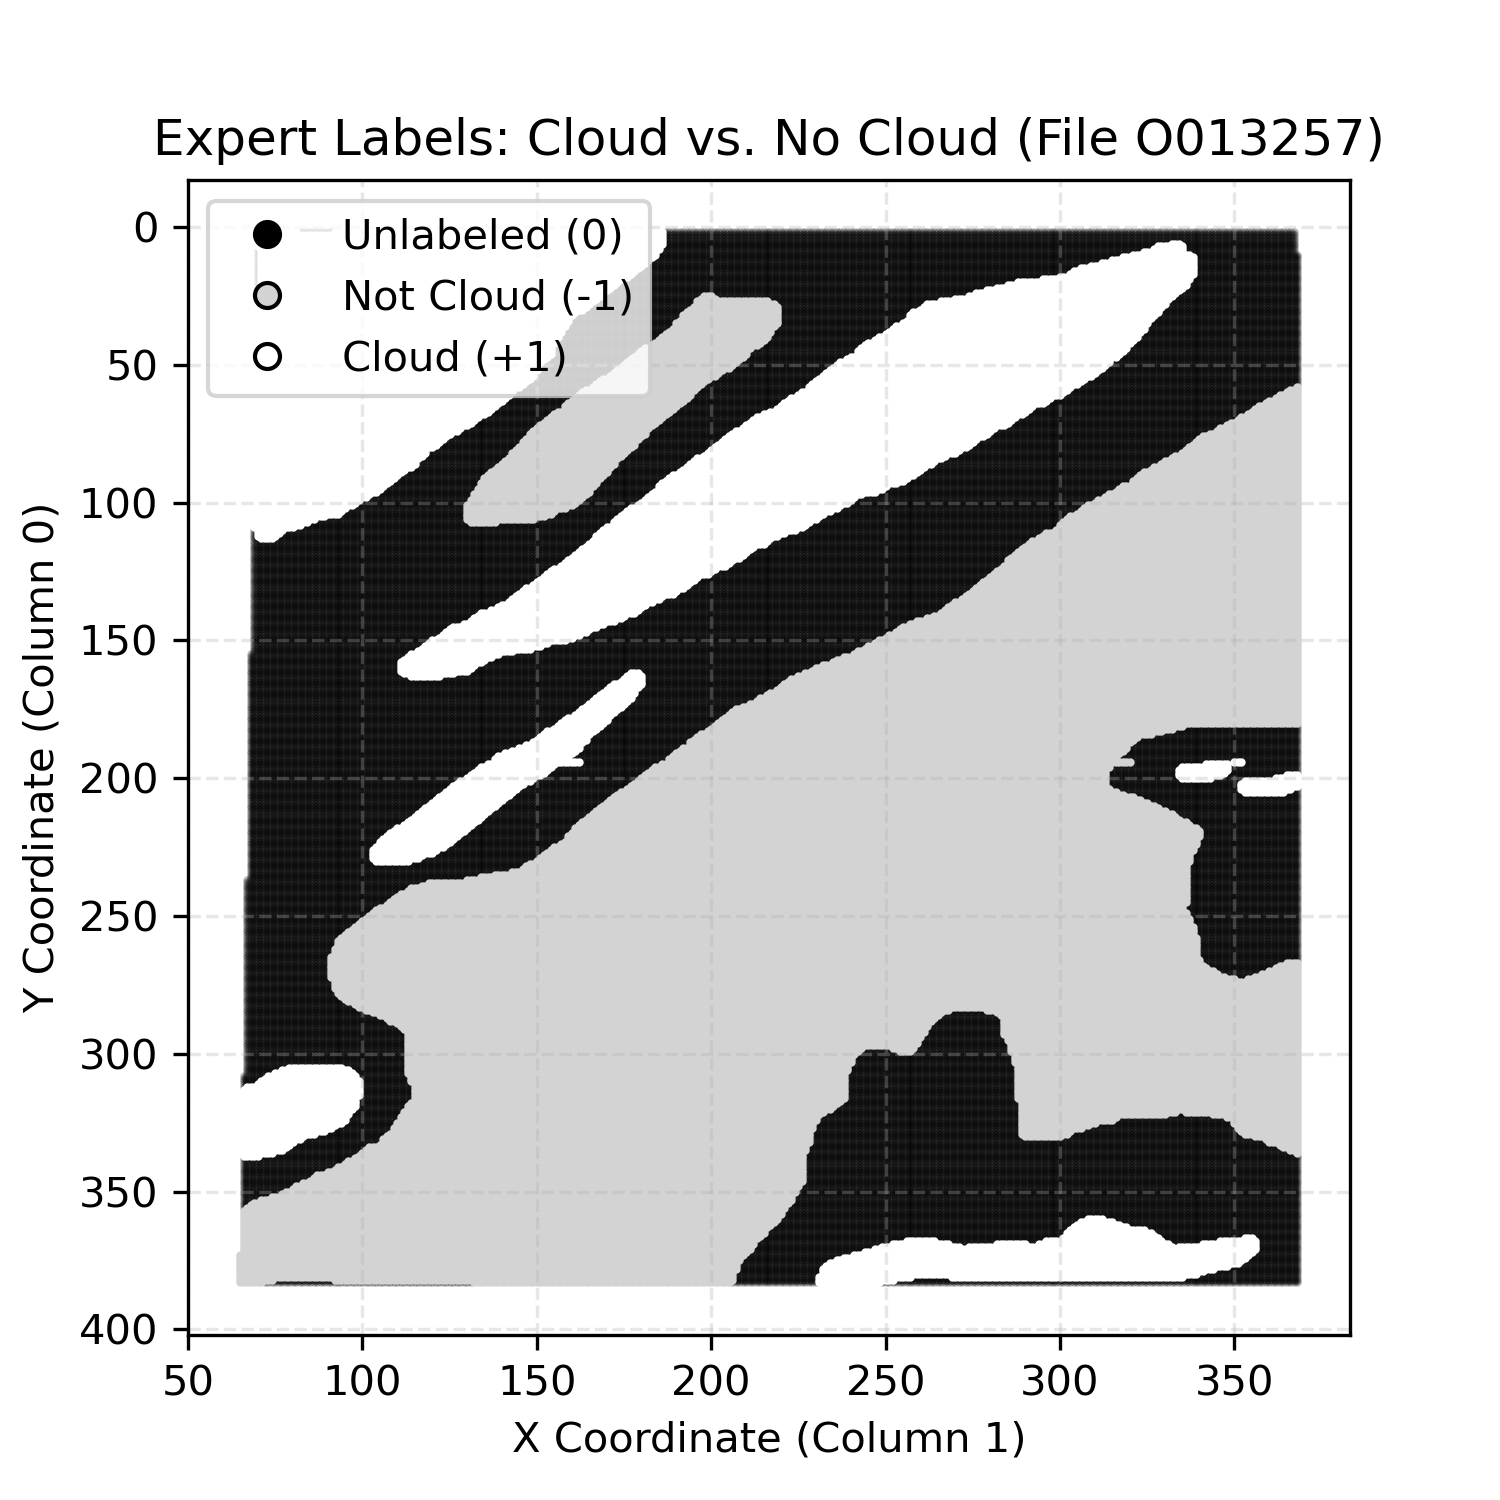
\includegraphics[width=\linewidth]{../figs/O013257.png}
        \caption{Image O013257}
    \end{subfigure}
    \hfill
    \begin{subfigure}{0.3\linewidth}
        \centering
        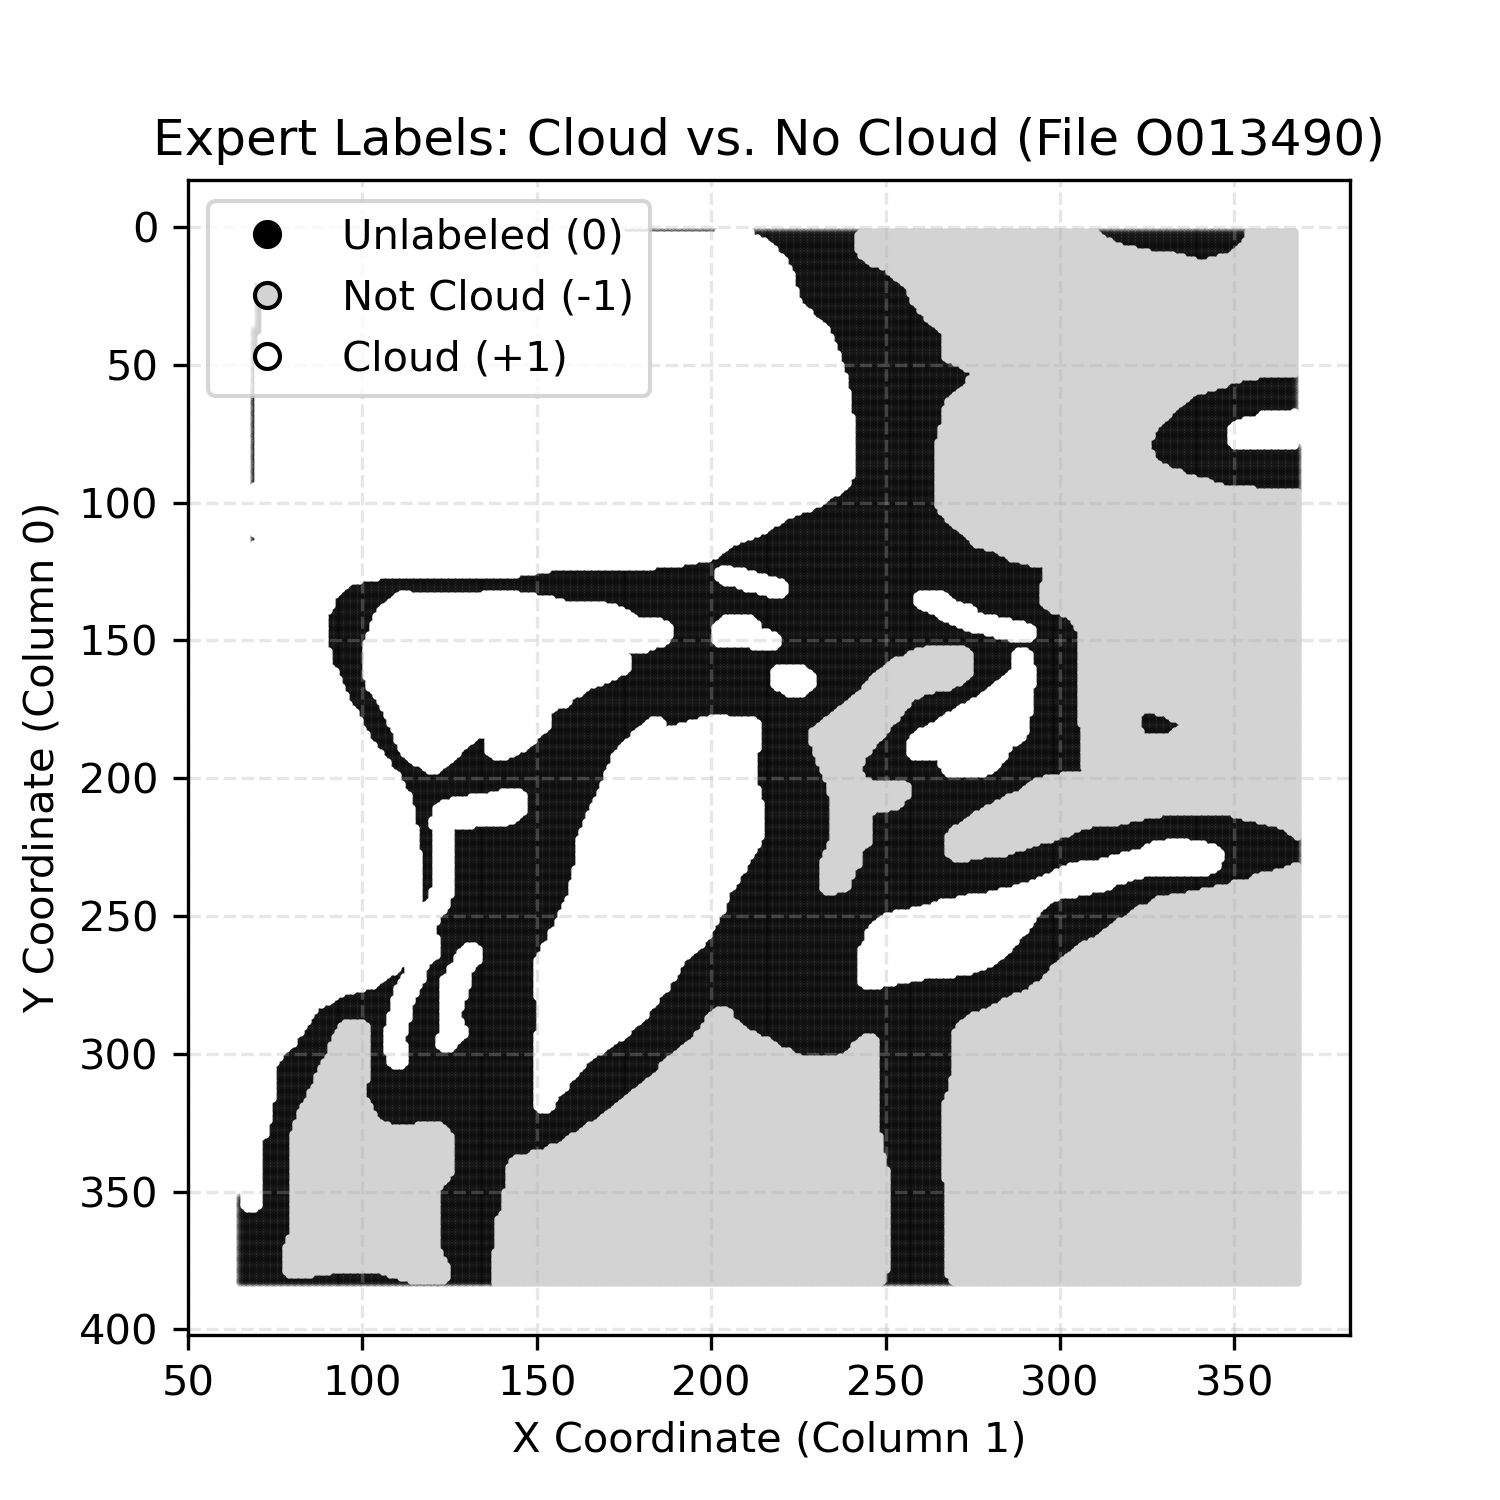
\includegraphics[width=\linewidth]{../figs/O013490.png}
        \caption{Image O013490}
    \end{subfigure}

    \caption{Plots of expert labels for presence and absence of clouds}
    \label{fig:three_labeled_images}
\end{figure}

\subsection{Feature Exploration}

Evaluating the radiance data, we found that multi-angle radiances are strongly correlated within an image. When restricting to cloud pixels, the radiance-angle correlation slightly decreases compared to non-cloud pixels. This indicates increased scattering properties of liquid and ice-water cloud particles over snow and ice covered surfaces. 


\begin{figure}[htbp]
\centering

\begin{minipage}[t]{0.48\textwidth}

\centering
\vspace{0.2pt}

\textbf{Pairwise correlations of multi-angle radiance features for cloud and non-cloud pixels.}

\vspace{1cm}

\begin{tabular}{lccc}
\toprule
Pair & Cloud & Non-Cloud & Diff \\
\midrule
DF--CF & 0.940 & 0.966 & -0.025 \\
DF--BF & 0.898 & 0.916 & -0.018 \\
DF--AF & 0.871 & 0.820 & 0.051 \\
DF--AN & 0.860 & 0.705 & 0.155 \\
CF--BF & 0.976 & 0.975 & 0.000 \\
CF--AF & 0.959 & 0.906 & 0.053 \\
CF--AN & 0.948 & 0.813 & 0.136 \\
BF--AF & 0.991 & 0.971 & 0.020 \\
BF--AN & 0.983 & 0.905 & 0.077 \\
AF--AN & 0.995 & 0.978 & 0.017 \\
\bottomrule
\end{tabular}

\vspace{1.5cm}
\textbf{(a)} Correlation summary
\end{minipage}
\hfill
\begin{minipage}[t]{0.48\textwidth}
\vspace*{0pt}
\centering

\textbf{Radiance relationship between DF and AN viewing angles.}

\vspace{0.4cm}

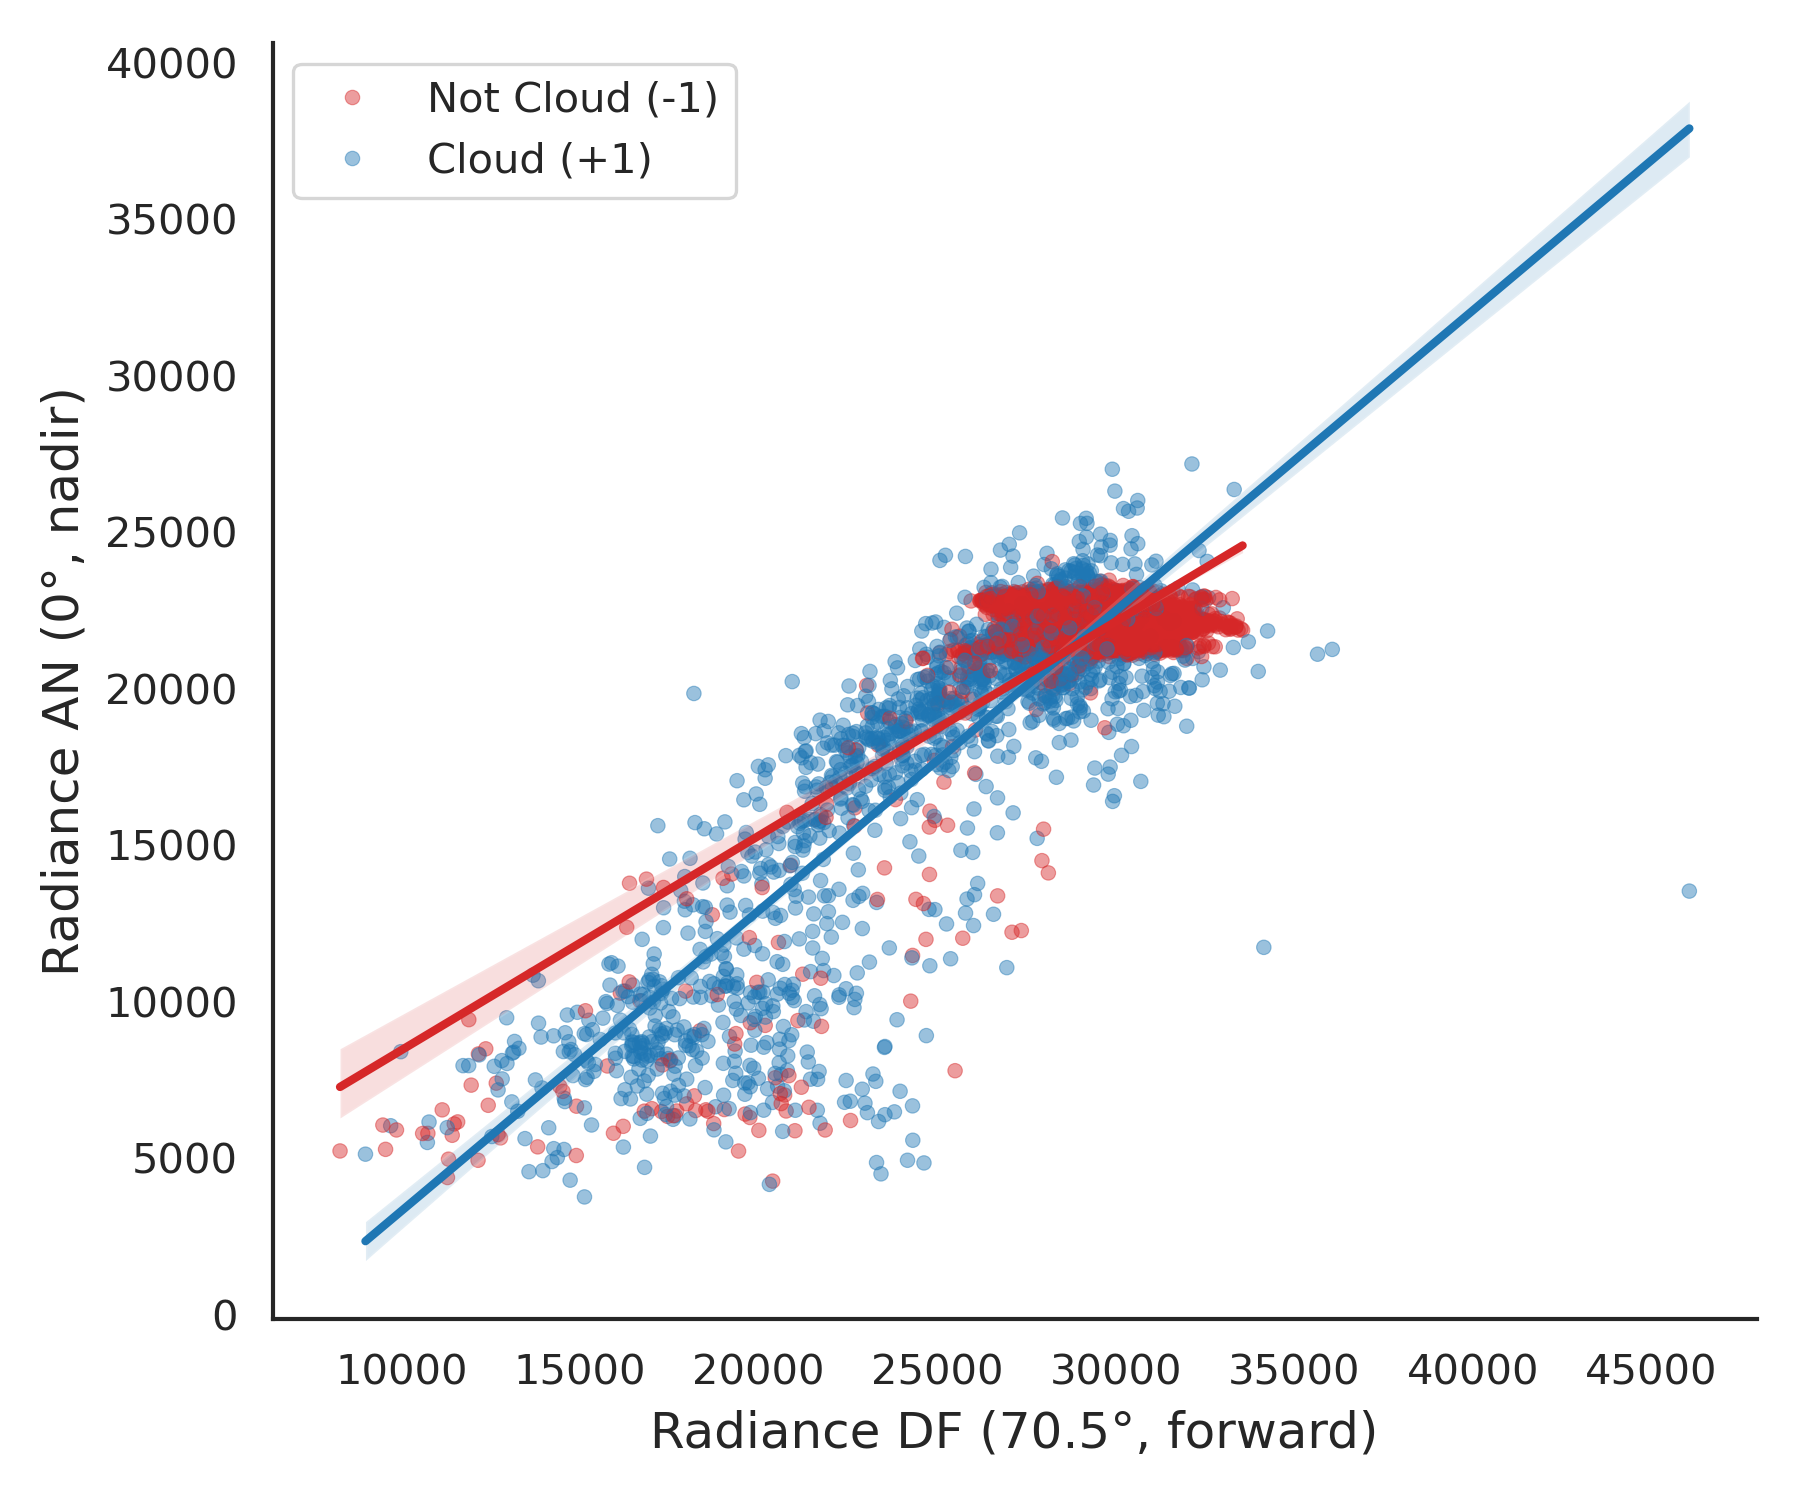
\includegraphics[width=\linewidth]{../figs/radiance_DF_vs_AN_scatter.png}

\vspace{0.5cm}
\textbf{(b)} Radiance relationship (DF vs AN)
\end{minipage}

\caption{Quantitative and visual comparison of multi-angle radiance relationships (Image O013257). (a) Pairwise correlations indicate strong dependence across viewing angles, with slightly weaker correlations for cloud pixels. (b) Scatter plot of forward (DF) and nadir (AN) radiance shows greater variability for cloud pixels.}
\label{fig:radiance_combined}
\end{figure}


The engineered features outlined in the paper  help to reveal clear class differences. 


Restricting to the labeled data, NDAI and SD were higher for cloud pixels than non-cloud pixels with statistically strong results following two-sample t-test evaluation. One note on the engineered features: NDAI, SD, and CORR are not highly linearly correlated with each other, so they likely capture different aspects of the scene. For classifying the cloud label, a single feature may be insufficient, but the combination will be a good trial.

\begin{figure}[htbp]
    \centering
    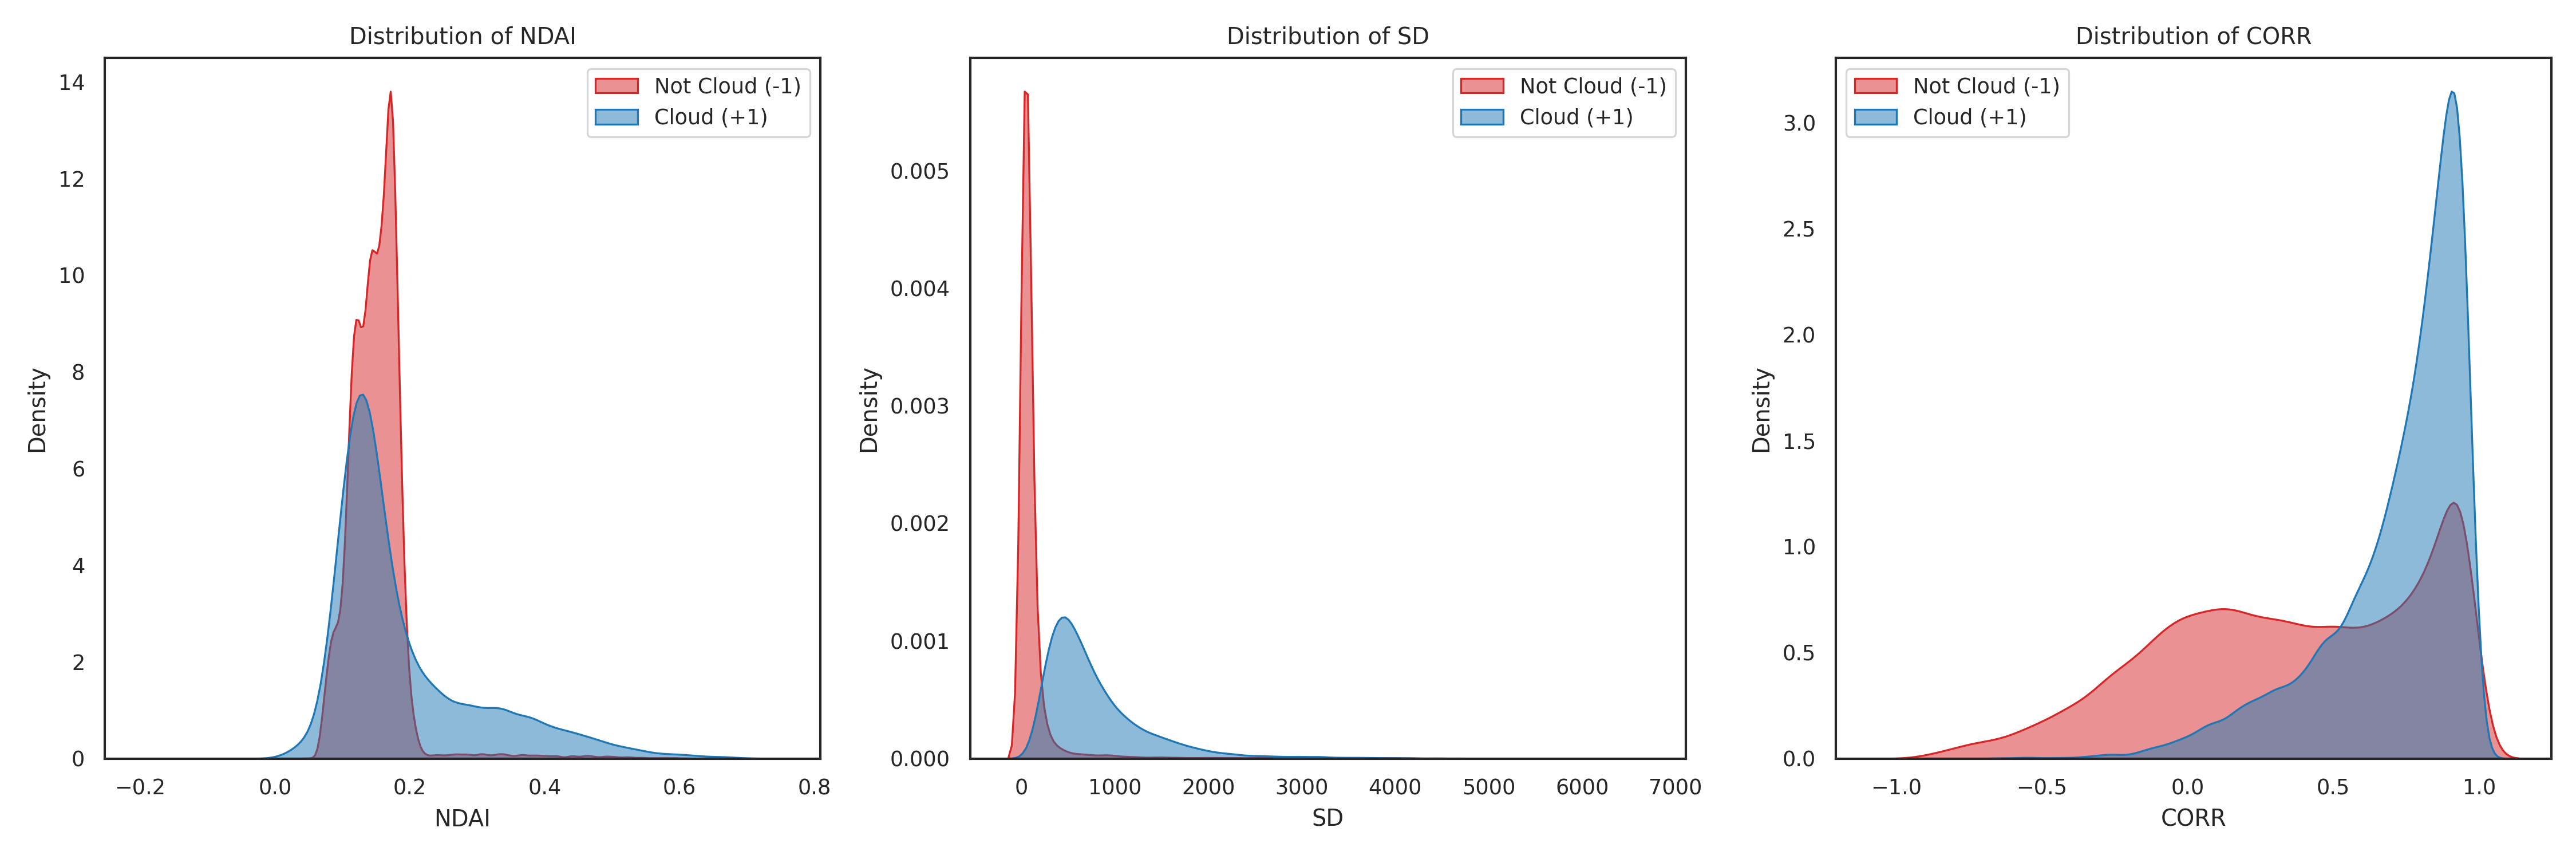
\includegraphics[width=1\linewidth]{../figs/KDE_expert_features.png}
    \caption{Distribution of NDAI, SD, and CORR for cloud and non-cloud pixels.}
    \label{fig:distribution-for-three-features}
\end{figure}

\subsection{Splitting}


Basically, for spatial data, random splitting introduces a risk of data leakage, since neighboring pixel units tend to share similar patterns. This can lead to overly optimistic performance in the validation and test sets. Therefore, we propose two splitting strategies: image-based splitting and quadrant-based splitting.

\subsubsection{Image-based splitting}

The safest approach is to assign one entire image to each split. To ensure sufficient training data, we allocate the image with the most labeled data points to the training set, the image with the fewest to the validation set, and the remaining image to the test set.


However, this image-level splitting results in a relatively small training set, which can limit model performance, especially for more complex models such as modern ensemble methods. Therefore, we introduce an alternative splitting strategy that trades off between sample size and the risk of data leakage.

\subsubsection{Quadrant-based splitting} \label{sec: quadrant-based}
Within the training images, each image was divided into four quadrants (Q1--Q4) based on the median values of the $x$ and $y$ coordinates specific to that image. The quadrants were defined as follows:

\begin{itemize}
    \item Q1: pixels with $x \leq \mathrm{median}_x$ and $y \leq \mathrm{median}_y$
    \item Q2: pixels with $x > \mathrm{median}_x$ and $y \leq \mathrm{median}_y$
    \item Q3: pixels with $x \leq \mathrm{median}_x$ and $y > \mathrm{median}_y$
    \item Q4: pixels with $x > \mathrm{median}_x$ and $y > \mathrm{median}_y$
\end{itemize}

This quadrant-based structure enables spatial analysis and offers a consistent framework for evaluating model performance across different regions of each image during cross-validation. Before training and testing, all unlabeled pixels were removed, keeping only those with confirmed expert labels (cloud or non-cloud). Additionally, after assigning quadrants, the spatial coordinates $(x, y)$ and image identifiers were excluded from the feature set, as they do not contribute meaningful general information for the cloud detection task. Overall, this strategy ensures a clear separation between training and testing data, reduces the risk of data leakage, and allows for a more reliable assessment of how well the model generalizes to entirely unseen spatial regions.

This strategy may introduce non-negligible spatial leakage, since neighboring regions share overlapping contextual information due to feature engineering. Therefore, results based on quadrant-based splitting should be interpreted with caution, and image-level splitting remains the most reliable evaluation for generalization.


\subsection{Cleaning}

\begin{figure}[htbp]
    \centering
    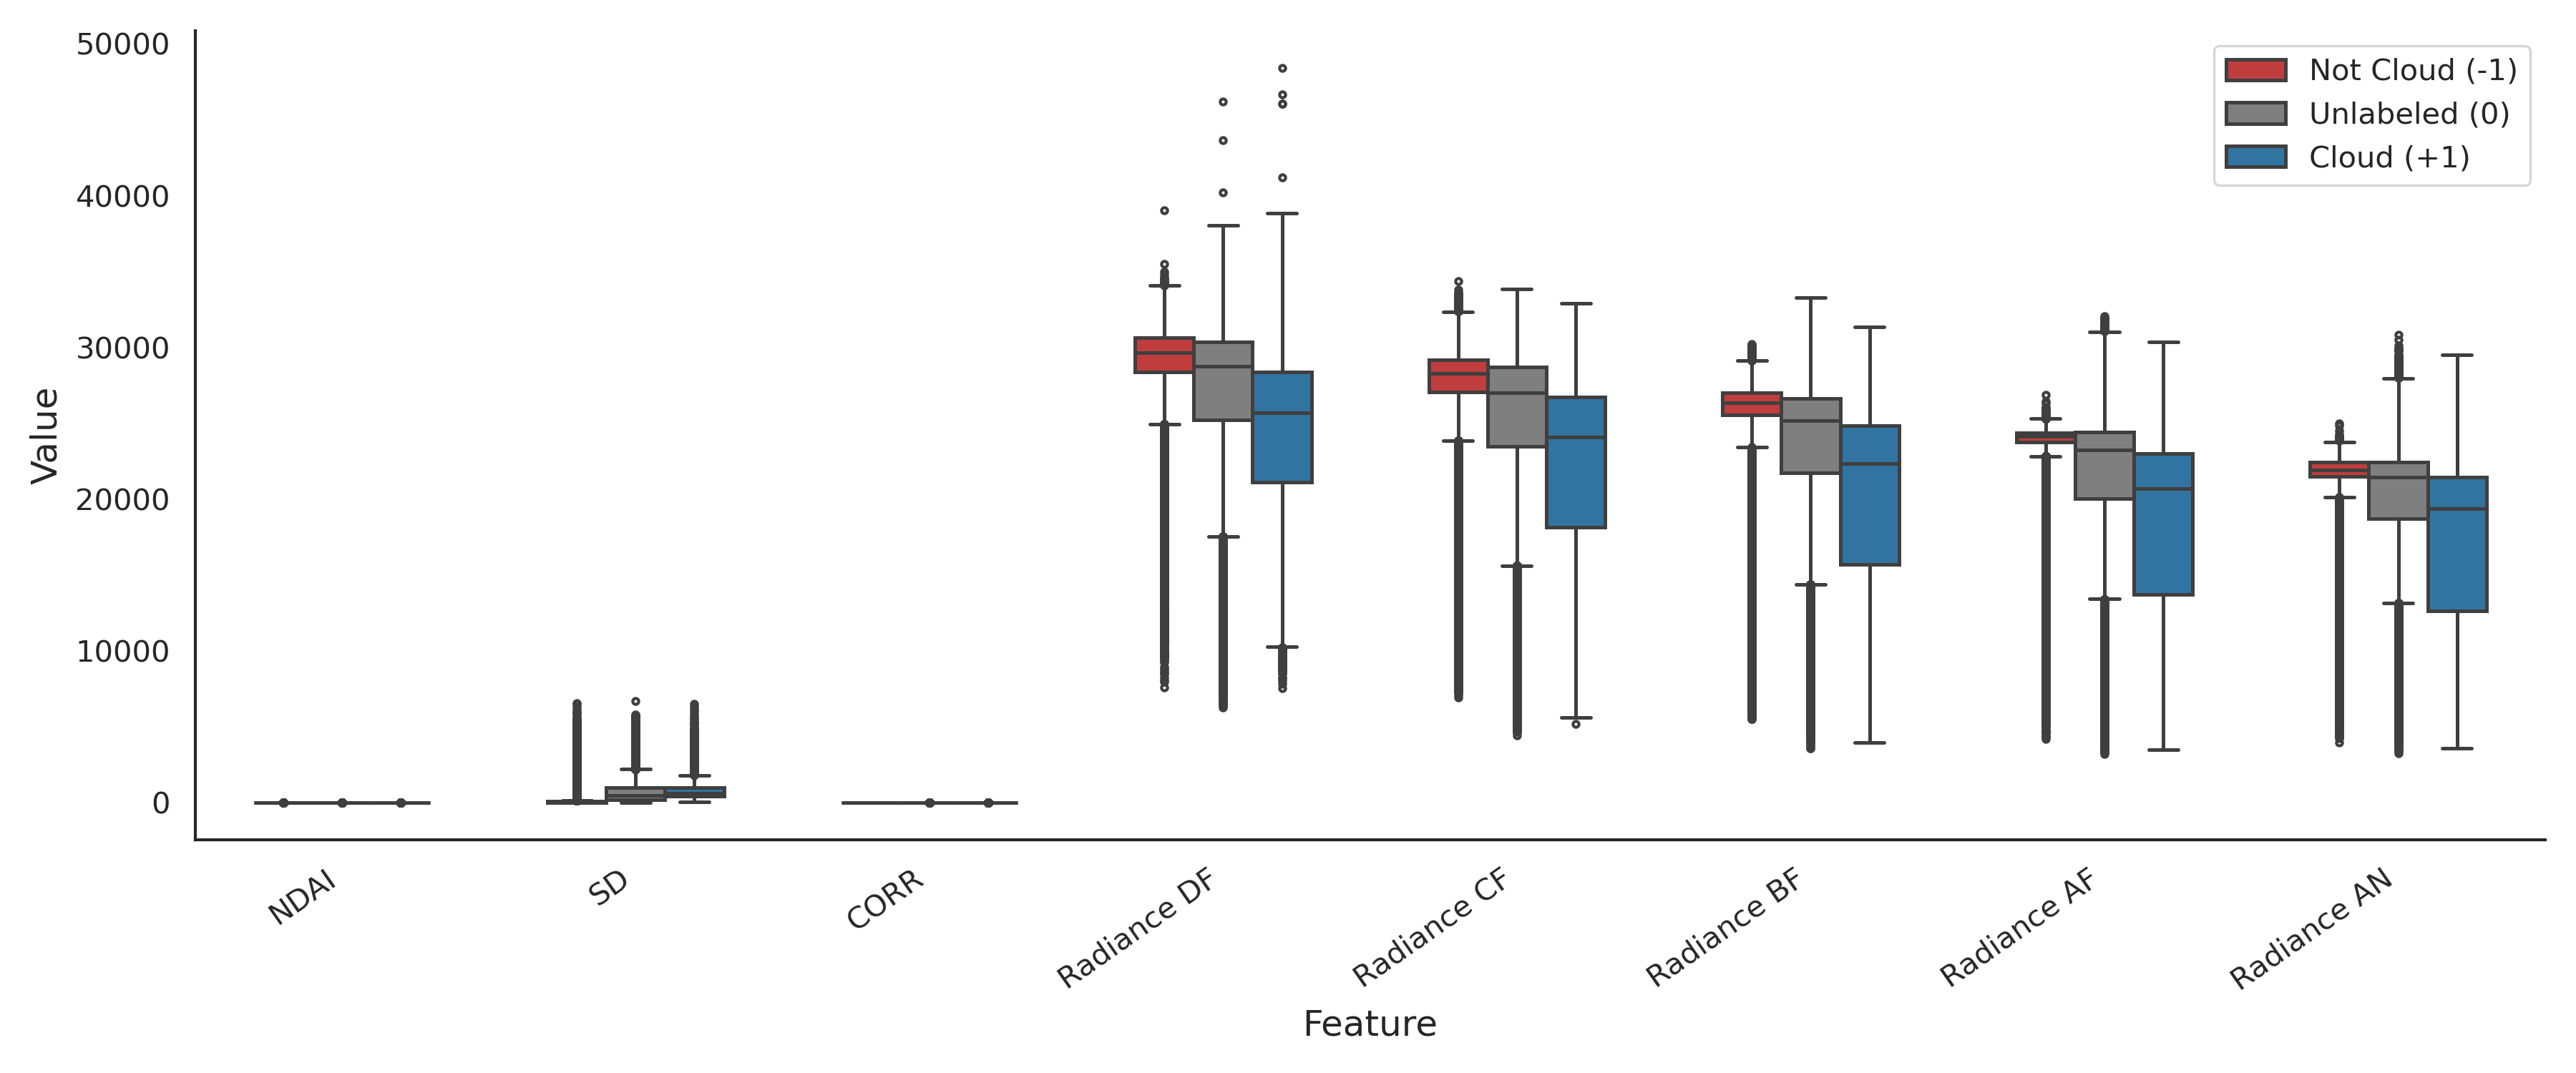
\includegraphics[width=1\linewidth]{../figs/boxplot_features_by_label.png}
    \caption{Boxplots of radiance and spatial features for cloud and non-cloud pixels.}
    \label{fig:boxplots-feature}
\end{figure}


As shown in Figure~\ref{fig:boxplots-feature}, the main issue with the data was the significant presence of outliers that skewed the impact of various features. Our data preparation included removing outliers based on the Z-score of the designated training image. Additionally, the data were optionally scaled after splitting and unlabeled data was dropped. Each image was also checked for duplicate rows (based on the x and y coordinate columns) and sanity checks were performed for each of the features.   


\section{Feature Engineering}
\subsection{Feature Importance Analysis}

Before proceeding to modeling and pixel classification, we first examine the current set of features in our dataset, with particular attention to their relative importance. One way to assess feature importance is by using a CART model. This model constructs a decision tree with a binary branching structure, which makes it relatively simple to interpret. For this reason, it is suitable for an initial evaluation of feature relevance. To maintain a balance between model complexity and interpretability, the tree depth was limited to four levels.

Figure ~\ref{fig:cart_base} presents the resulting decision tree based on the original dataset. It clearly shows that the features SD and CORR—identified as expert features—have the highest importance, while the remaining features contribute less significantly.

It can also be observed that this simple CART model already achieves an accuracy of 95\%, which is an impressive result for such a straightforward approach. However, in the following chapters, we will further enhance the feature set through additional feature engineering. Finally, we will construct a corresponding CART model to compare the performance of the original dataset with that of the extended dataset containing the new features.

\begin{figure}[H]
    \centering
    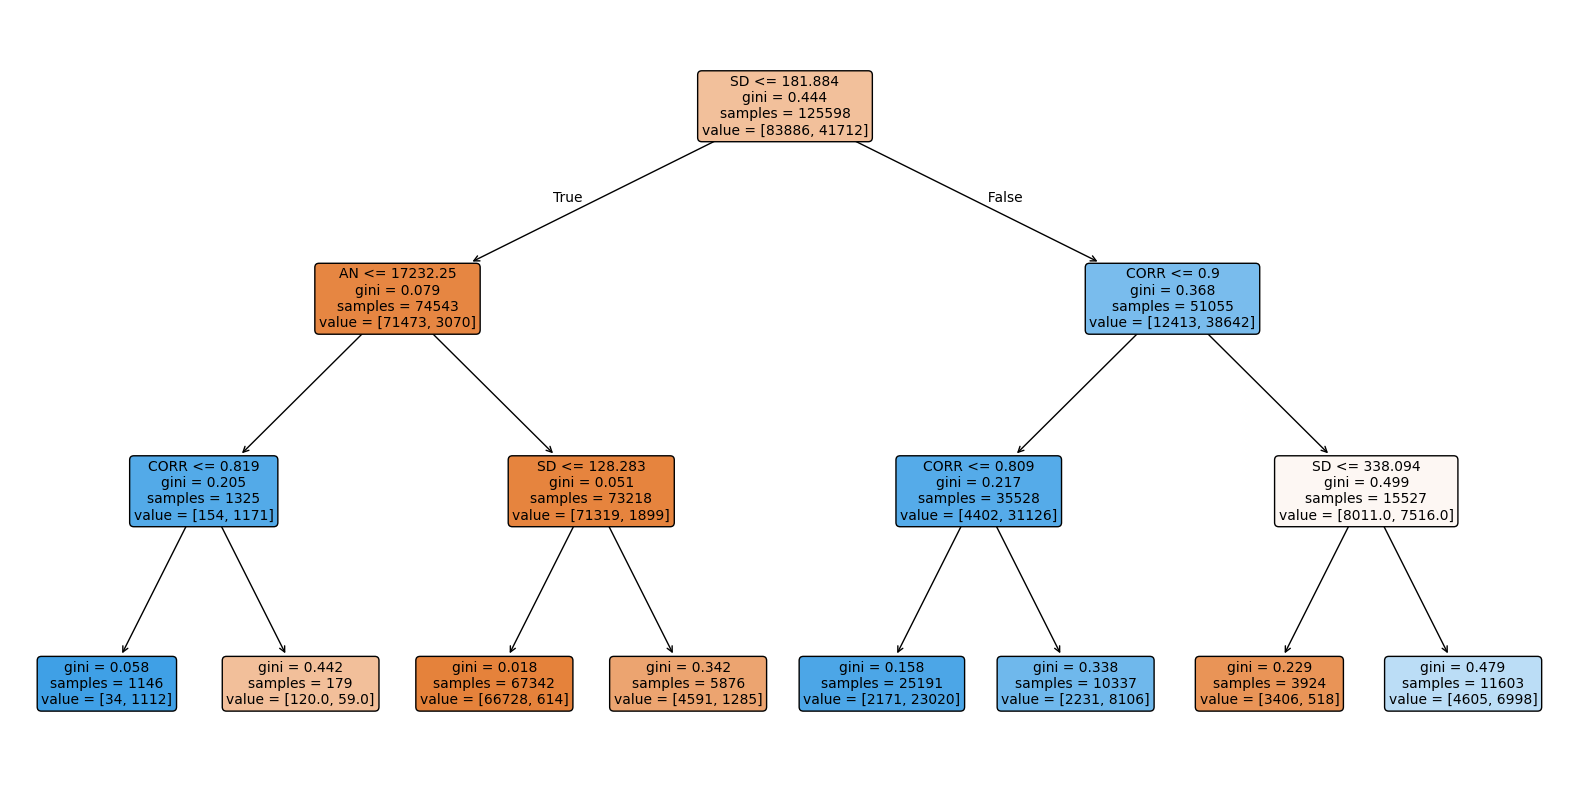
\includegraphics[width=1\linewidth]{../figs/cart_base.png}
    \caption{CART model before feature engineering}
    \label{fig:cart_base}
\end{figure}

\subsection{Feature Creation}

We now take a closer look at how to enhance the dataset by introducing additional features to improve prediction performance. This approach is motivated by insights from the exploratory data analysis (EDA), which revealed that clouds tend to appear in large clusters that form wave-like fronts. As a result, neighboring pixels are likely to share similar characteristics, meaning that incorporating information from the surrounding area can provide a richer representation of each individual data point.

However, this approach introduces an important constraint: since each data point now includes information from its surroundings, a random train-test split is no longer appropriate. Instead, entire regions or images must be assigned exclusively to either the training or testing set to avoid data leakage.

In terms of implementation, for each original feature (such as SD, CORR, NDAI, DF, CF, BF, AF, and AN), additional features are generated by computing summary statistics—mean, minimum, and maximum—over different neighborhood sizes. Specifically, three window sizes were considered: 3×3, 5×5, and 9×9. For the largest window, these statistics are calculated using the 80 surrounding pixels.

As a result, each original feature is expanded into multiple new features. For example, the NDAI feature is transformed into nine additional features, such as NDAI\_3\_Mean, NDAI\_3\_Min, NDAI\_3\_Max, NDAI\_5\_Mean, and so on up to NDAI\_9\_Max. Consequently, the dataset grows to over 80 features, significantly increasing its dimensionality. This expanded feature space captures environmental context but may require further feature selection or dimensionality reduction during modeling.

\subsection{Summary}

To summarize the feature engineering process:  we observed that the original features, together with the CART model, already achieved relatively strong performance, with SD and CORR being particularly influential. Also, we introduced additional features derived from neighboring pixels and an autoencoder. To conclude this part, we re-evaluated feature importance using the CART model to examine how these additions affected the results.

The following figure presents the outcomes based on both the original and the newly engineered features. It shows that cluster separation is only weakly driven by the original features, while the newly introduced features play a dominant role. 

In particular, features derived from surrounding pixels appear most important and are positioned near the top of the decision tree. 
% In contrast, autoencoder-based features are also utilized but tend to appear deeper in the tree, indicating a lower relative importance.

\begin{figure}[H]
    \centering
    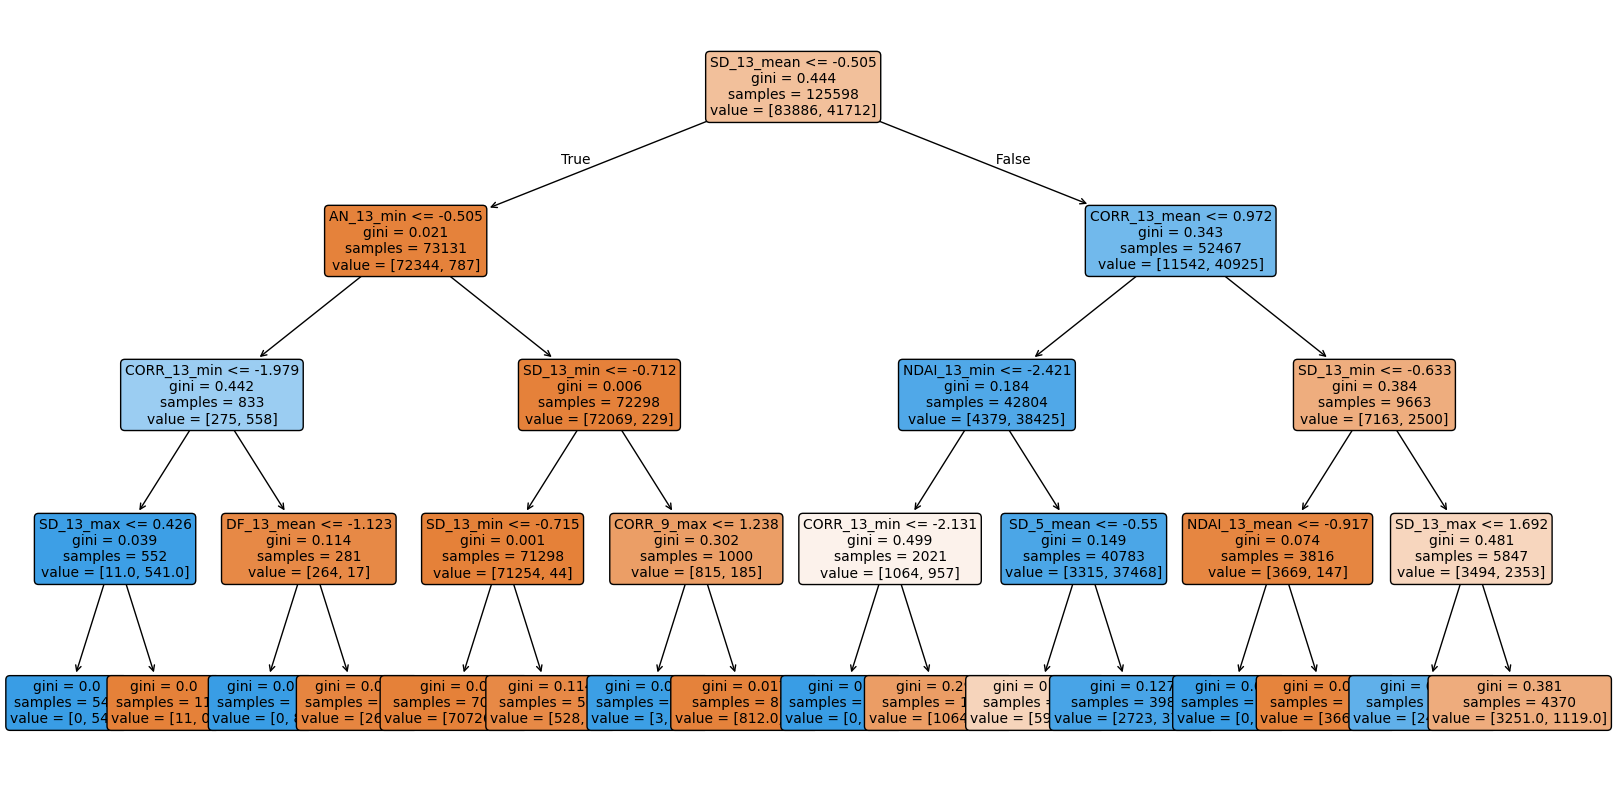
\includegraphics[width=1\linewidth]{../figs/cart_new.png}
    \caption{CART model after feature engineering}
    \label{fig:cart_new}
\end{figure}

Overall, this analysis shows that the feature engineering carried out in this chapter has significantly expanded and refined the dataset. Importantly, the results confirm that the steps introduced in the Section 3.2 contributed highly informative features, which are expected to simplify the classification task and lead to substantially improved performance in subsequent models.

\section{Feature Engineering — Transfer Learning}

\subsection{Overview of Transfer Learning}

One major challenge in cloud prediction is the limited number of labeled data, which hinders the training of prediction models. As a complementary approach to previous feature engineering approaches, we explore transfer learning to address this issue, which makes better use of abundant unlabeled data while keeping the final model focused on the labeled data.

In this section, we develop a two-stage transfer learning pipeline based on autoencoders. We first pretrain an autoencoder on 162 unlabeled images to learn general cloud representations, and then finetune the model on 3 labeled images to adapt it for the downstream supervised task. 8 embedding features are derived from the encoder and fed into models for cloud prediction.

In the pretraining stage, an autoencoder is training on unlabeled image patches. At each epoch, the model weights are updated on the basis of the MSE reconstruction loss on the training set, and the performance is evaluated on the validation set. The weights with the best validation performance are saved as the pretrained model for the next stage. We set the maximum number of epochs to 100, which is sufficient for the loss to stabilize.

In the finetuning stage, the model weights are initialized from the pretrained model and further updated on the labeled image patches. To stabilize the finetuning process and avoid overfitting, we use a smaller learning rate (1e-5) compared to pretraining. Moreover, the number of finetuning epochs is set to 20, which is sufficient for the loss to stabilize without overfitting.

\begin{figure}[h]
    \centering
    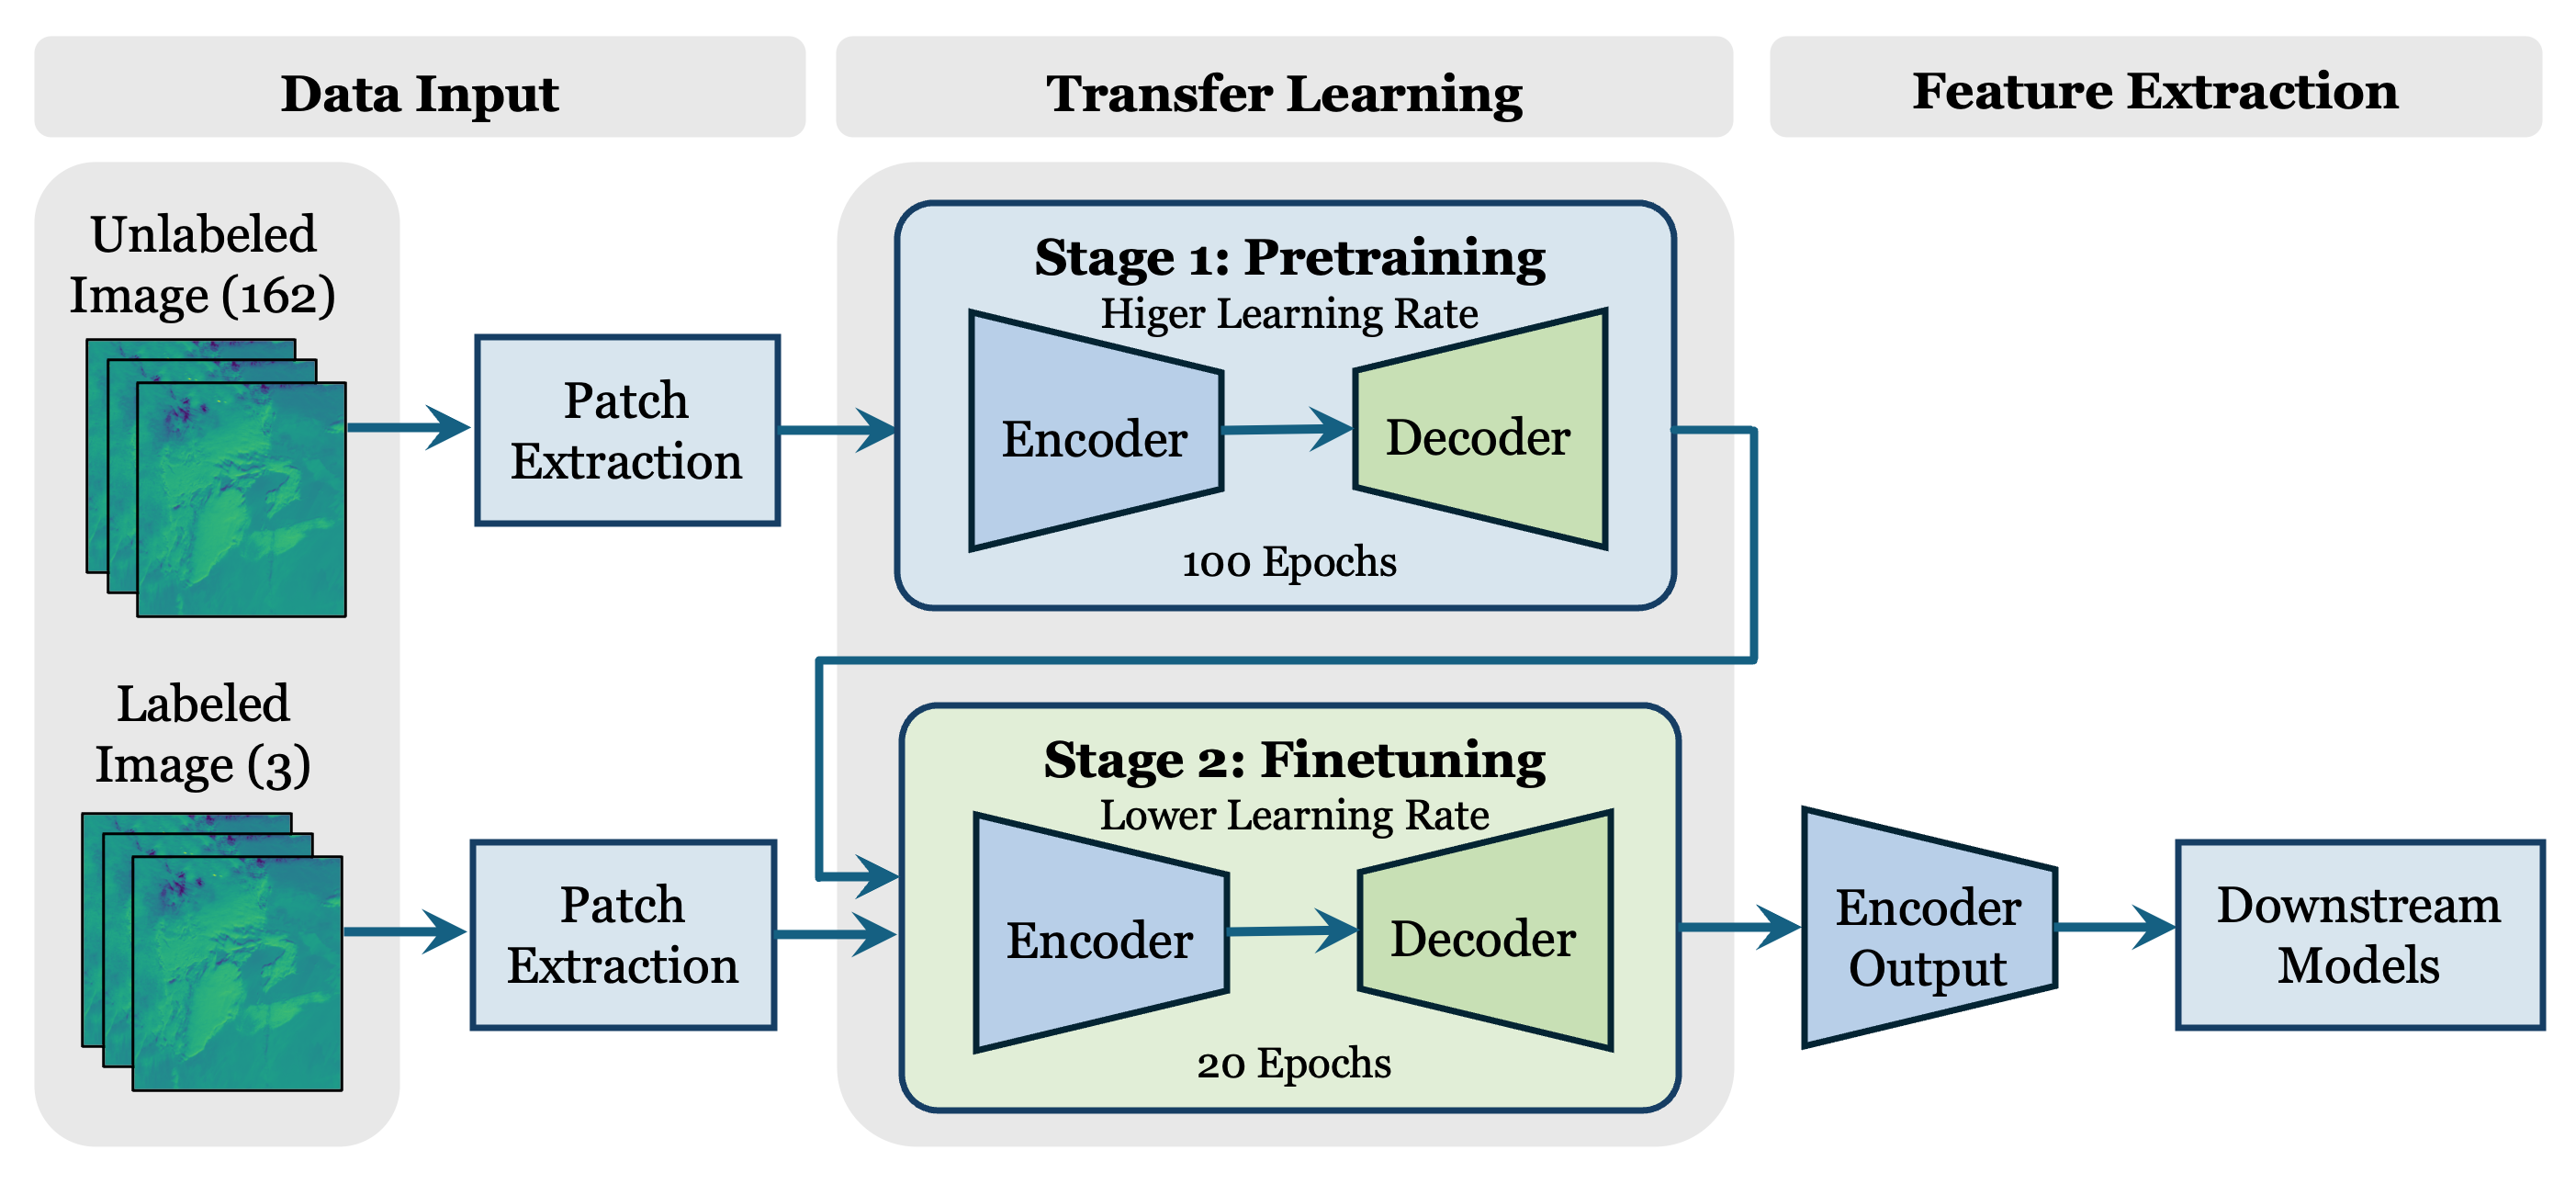
\includegraphics[width=0.7\linewidth]{../figs/transfer_learning_pipeline.png}
    \caption{Transfer learning pipeline}
    \label{fig:final_ae_arch}
\end{figure}

For the choice of optimizer, while the baseline suggests using Adam, we adopt AdamW as the optimizer, since it decouples weight decay from the gradient update and often leads to improved generalization in practice \cite{loshchilov2017decoupled}. The weight decay is set to 1e-5 to regularize the model and prevent overfitting. The batch size is set to 4096, which is a good balance between computational efficiency and convergence stability.

The choice of model architecture and hyperparameters is based on experiments and benchmarking results on the test set, which will be described in later subsections.


\subsection{Data Preprocessing and Splitting}

The image data used for transfer learning is processed at the patch level. For each pixel in the original image, we extract a $9 \times 9$ patch centered around it. For pixels near the borders, we apply reflection-padding to maintain consistent patch sizes. This design allows the autoencoder to learn local spatial patterns that are important for cloud representation.

However, one challenge in this approach is the potential for data leakage. Since neighboring patches from the same image share pixels, they are highly correlated with each other. If we conduct patch-level train-test splitting randomly, we risk having patches from the same image in both sets. This would lead to overly optimistic reconstruction results due to data leakage. To address this issue, we borrow the idea of group-based splitting and perform data splits at the image level. All patches derived from a single image are assigned to the same set.

Following this strategy, we randomly split the 162 unlabeled images into training, validation, and test sets before the pretraining stage. To ensure reproducibility, we use a fixed random seed. The split ratio is 80\% for training, 10\% for validation, and 10\% for testing. Table~\ref{tab:transfer_split} summarizes the image-level split used in our transfer learning pipeline.


\begin{table}[h]
\centering
\caption{Transfer learning data splitting}
\label{tab:transfer_split}
\renewcommand{\arraystretch}{2}
\setlength{\tabcolsep}{8pt}
\begin{tabular}{c c c c c l}
\hline
Stage & Set & Source & \# Images & \# Patches & Usage \\
\hline
Pretrain & Train & Unlabeled &
\makecell[c]{128\\{\footnotesize(79.50\%)}} &
\makecell[c]{14,779,819\\{\footnotesize(79.51\%)}} & AE Training \\[3pt]

Pretrain & Validation & Unlabeled &
\makecell[c]{16\\{\footnotesize(9.94\%)}} &
\makecell[c]{1,847,708\\{\footnotesize(9.94\%)}} & AE checkpoint selection\\[3pt]

Pretrain & Test & Unlabeled &
\makecell[c]{17\\{\footnotesize(10.56\%)}} &
\makecell[c]{1,962,097\\{\footnotesize(10.55\%)}} & AE comparison \\[3pt]

Finetune & Train & Labeled &
\makecell[c]{3} &
\makecell[c]{345,005} & AE finetuning \\
\hline
\end{tabular}
\end{table}


Notice that the data splitting strategy is different for pretraining and finetuning stages. For finetuning, since we only have 3 labeled images, we do not create a separate validation set to avoid instability. Instead, we use all 3 labeled images for training. The potential risk of overfitting is mitigated by using a smaller learning rate and limiting the number of finetuning epochs, as mentioned in the previous subsection.

The test set is kept fully unseen during both pretraining and finetuning stages. This ensures that the evaluation of reconstruction performance is unbiased. Moreover, we keep the test image IDs fixed across all experiments to ensure that differences in reconstruction metrics are due to model design and hyperparameters rather than changes in evaluation samples.



\subsection{Architecture Comparison}

In this section, we compare the reconstruction performance of different autoencoder architectures. We experiment with both MLP-based and convolutional autoencoders, as well as variations in depth, width, and denoising layer. For each architecture design, we evaluate both the pretrain and finetuned models using the test set.

For the realization of denoising layer, we add Gaussian noise to the input patches during training, which encourages the model to learn more robust representations. The noise level is set to a standard deviation of 0.05, which is a common choice for denoising autoencoders.

For the realization of MLP autoencoder, we use a simple architecture with 2/3 fully connected layers in the encoder and the same number of layers in the decoder. The number of hidden units is set to 128/256/384 for the first layer and halved for each subsequent layer.

For the realization of convolutional autoencoder, we use a simple architecture with 2/3 convolutional layers in the encoder and the same number of transposed convolutional layers in the decoder. The kernel size is set to 3, and the number of channels is set to 32/48 for the first layer and doubled for each subsequent layer.

To ensure comparability across different architecture designs, we fix the data splitting strategy and training protocol for all experiments. The same train/validation/test sets are used for all models. Four reconstruction metrics are reported for reconstruction evaluation, including MSE, RMSE, MAE, and PSNR. The primary metric for comparison is MSE, as it directly reflects the optimization objective of the autoencoder. The other metrics are included to provide additional evaluation on reconstruction quality.

\begin{table*}[t]
\centering
\caption{Architecture comparison on pretrained models}
\label{tab:arch_comp_pretrain}
\scriptsize
\setlength{\tabcolsep}{4pt}
\begin{tabular}{c c c c c c c c}
\toprule
Exp & Type & Structure & Denoising ($\sigma$) & MSE $\downarrow$ & RMSE $\downarrow$ & MAE $\downarrow$ & PSNR $\uparrow$ \\
\midrule
018 & MLP  & [128,64]       & No         & 0.127104 & 0.356516 & 0.210432 & 33.363029 \\
019 & MLP  & [128,64]       & Yes (0.05) & 0.126618 & 0.355835 & 0.209366 & 33.379653 \\
020 & MLP  & [256,128,64]   & No         & 0.123609 & 0.351581 & 0.207619 & 33.484120 \\
021 & MLP  & [256,128,64]   & Yes (0.05) & 0.124315 & 0.352584 & 0.207389 & 33.459376 \\
026 & MLP  & [384,192,96]   & No         & 0.123447 & 0.351350 & 0.206265 & 33.489824 \\
027 & MLP  & [384,192,96]   & Yes (0.05) & 0.122865 & 0.350521 & 0.206102 & 33.510338 \\
\midrule
022 & Conv & [32,64]        & No         & 0.131459 & 0.362573 & 0.214654 & 33.216718 \\
023 & Conv & [32,64]        & Yes (0.05) & 0.132665 & 0.364233 & 0.215150 & 33.177047 \\
024 & Conv & [32,64,128]    & No         & 0.121799 & 0.348997 & 0.207415 & 33.548183 \\
025 & Conv & [32,64,128]    & Yes (0.05) & 0.122823 & 0.350461 & 0.209127 & 33.511831 \\
028 & Conv & [48,96,192]    & No         & \textbf{0.118697} & \textbf{0.344524} & \textbf{0.204885} & \textbf{33.660221} \\
029 & Conv & [48,96,192]    & Yes (0.05) & 0.119609 & 0.345845 & 0.205780 & 33.626980 \\
\bottomrule
\end{tabular}
\end{table*}


\begin{table*}[t]
\centering
\caption{Architecture comparison on finetuned models}
\label{tab:arch_comp_finetune}
\scriptsize
\setlength{\tabcolsep}{4pt}
\begin{tabular}{c c c c c c c c}
\toprule
Exp & Type & Structure & Denoising ($\sigma$) & MSE $\downarrow$ & RMSE $\downarrow$ & MAE $\downarrow$ & PSNR $\uparrow$ \\
\midrule
018 & MLP  & [128,64]       & No         & 0.126417 & 0.355552 & 0.208871 & 33.386569 \\
019 & MLP  & [128,64]       & Yes (0.05) & 0.123518 & 0.351451 & 0.206596 & 33.487317 \\
020 & MLP  & [256,128,64]   & No         & 0.122178 & 0.349540 & 0.205453 & 33.534679 \\
021 & MLP  & [256,128,64]   & Yes (0.05) & 0.121999 & 0.349283 & 0.205270 & 33.541075 \\
026 & MLP  & [384,192,96]   & No         & 0.121882 & 0.349116 & 0.204286 & 33.545223 \\
027 & MLP  & [384,192,96]   & Yes (0.05) & 0.120855 & 0.347642 & \textbf{0.203956} & 33.581967 \\
\midrule
022 & Conv & [32,64]        & No         & 0.129273 & 0.359545 & 0.213505 & 33.289557 \\
023 & Conv & [32,64]        & Yes (0.05) & 0.129355 & 0.359660 & 0.213203 & 33.286777 \\
024 & Conv & [32,64,128]    & No         & 0.120920 & 0.347735 & 0.206687 & 33.579645 \\
025 & Conv & [32,64,128]    & Yes (0.05) & 0.120773 & 0.347524 & 0.206608 & 33.584919 \\
028 & Conv & [48,96,192]    & No         & 0.118591 & 0.344371 & 0.205135 & 33.664100 \\
029 & Conv & [48,96,192]    & Yes (0.05) & \textbf{0.118357} & \textbf{0.344031} & 0.204616 & \textbf{33.672664} \\
\bottomrule
\end{tabular}
\end{table*}

The architecture comparison results are summarized in Table~\ref{tab:arch_comp_pretrain} for pretrained models and Table~\ref{tab:arch_comp_finetune} for finetuned models, respectively. We observe that convolutional autoencoders generally outperform MLP autoencoders with sufficient model depth and width, which is expected given the spatial nature of image data. Moreover, deeper and wider architectures tend to perform better, but the improvement is not always significant. The addition of denoising layer shows mixed results, which may depend on the specific architecture. For pretrained models, adding denoising layer slightly improves MLP autoencoders but slightly worsens convolutional autoencoders. For finetuned models, adding denoising layer consistently improves MLP autoencoders but has minimal impact on convolutional autoencoders.

Overall, the best performing model is the convolutional autoencoder with 3 layers and 48/96/192 channels with denoising layer (Conv [48,96,192], exp 029), which achieves the lowest MSE and RMSE and highest PSNR across all experiments. This architecture is selected and used for the subsequent hyperparameter tuning.

\begin{table*}[t]
\centering
\caption{Performance difference between finetuned and pretrained models
 (finetune - pretrain)}
\label{tab:delta_finetune_pretrain}
\scriptsize
\setlength{\tabcolsep}{4pt}
\begin{tabular}{c c c c c c c c}
\toprule
Exp & Type & Structure & Denoising ($\sigma$) & $\Delta$MSE & $\Delta$RMSE & $\Delta$MAE & $\Delta$PSNR \\
\midrule
018 & MLP  & [128,64]       & No         & -0.000687 & -0.000964 & -0.001561 & +0.023540 \\
019 & MLP  & [128,64]       & Yes (0.05) & -0.003100 & -0.004384 & -0.002770 & +0.107664 \\
020 & MLP  & [256,128,64]   & No         & -0.001431 & -0.002041 & -0.002166 & +0.050559 \\
021 & MLP  & [256,128,64]   & Yes (0.05) & -0.002316 & -0.003301 & -0.002119 & +0.081699 \\
026 & MLP  & [384,192,96]   & No         & -0.001565 & -0.002234 & -0.001979 & +0.055399 \\
027 & MLP  & [384,192,96]   & Yes (0.05) & -0.002010 & -0.002879 & -0.002146 & +0.071629 \\
\midrule
022 & Conv & [32,64]        & No         & -0.002186 & -0.003028 & -0.001149 & +0.072839 \\
023 & Conv & [32,64]        & Yes (0.05) & -0.003310 & -0.004573 & -0.001947 & +0.109730 \\
024 & Conv & [32,64,128]    & No         & -0.000879 & -0.001262 & -0.000728 & +0.031462 \\
025 & Conv & [32,64,128]    & Yes (0.05) & -0.002050 & -0.002937 & -0.002519 & +0.073088 \\
028 & Conv & [48,96,192]    & No         & -0.000106 & -0.000153 & +0.000250 & +0.003879 \\
029 & Conv & [48,96,192]    & Yes (0.05) & -0.001252 & -0.001814 & -0.001164 & +0.045684 \\
\midrule
\textbf{Mean} & - & - & - & \textbf{-0.001741} & \textbf{-0.002464} & \textbf{-0.001666} & \textbf{+0.060598} \\
\bottomrule
\end{tabular}
\end{table*}

Another noticeable observation is that the finetuned models generally outperform the pretrained models slightly. As shown in the Table~\ref{tab:delta_finetune_pretrain}, the improvement is more significant for MLP autoencoders than convolutional autoencoders, which may be because convolutional architectures are already well-suited for image data and benefit less from finetuning.


\subsection{Hyperparameter Tuning and Final Autoencoder Selection}

After fixing autoencoder family, we further conduct hyperparameter tuning on learning rate and dropout rate. We experiment with learning rates of [1e-3, 5e-4, 1e-4] and dropout rates of [0, 0.05, 0.1].

To increase the credibility of our results, the parameter tuning is conducted on two selected architectures, including Conv [32,64,128] and Conv [48,96,192], both with denoising layer. For each architecture, we evaluate the finetuned model performance on the test set under different hyperparameter combinations. The results are summarized in Table~\ref{tab:finetune_param_tuning}.

\begin{table*}[t]
\centering
\caption{Finetuned model performance under hyperparameter tuning}
\label{tab:finetune_param_tuning}
\scriptsize
\setlength{\tabcolsep}{5pt}
\begin{tabular}{c c c c c c c}
\toprule
Exp & Pretrain Dropout & Pretrain LR & MSE $\downarrow$ & RMSE $\downarrow$ & MAE $\downarrow$ & PSNR $\uparrow$ \\
\midrule
\multicolumn{7}{l}{\textbf{Panel A: Conv [32,64,128], denoising=True ($\sigma=0.05$)}}\\
\midrule
025 & 0.00 & $1\mathrm{e}{-3}$ & \textbf{0.120773} & \textbf{0.347524} & \textbf{0.206608} & \textbf{33.584919} \\
031 & 0.00 & $5\mathrm{e}{-4}$ & 0.121579 & 0.348681 & 0.207272 & 33.556044 \\
030 & 0.00 & $1\mathrm{e}{-4}$ & 0.126038 & 0.355018 & 0.211101 & 33.399610 \\
034 & 0.05 & $1\mathrm{e}{-3}$ & 0.131275 & 0.362319 & 0.222234 & 33.222794 \\
033 & 0.05 & $5\mathrm{e}{-4}$ & 0.131496 & 0.362624 & 0.221770 & 33.215491 \\
032 & 0.05 & $1\mathrm{e}{-4}$ & 0.131157 & 0.362157 & 0.221134 & 33.226694 \\
037 & 0.10 & $1\mathrm{e}{-3}$ & 0.149290 & 0.386381 & 0.244379 & 32.664304 \\
036 & 0.10 & $5\mathrm{e}{-4}$ & 0.152871 & 0.390987 & 0.248319 & 32.561380 \\
035 & 0.10 & $1\mathrm{e}{-4}$ & 0.148825 & 0.385778 & 0.243144 & 32.677865 \\
\midrule
\multicolumn{7}{l}{\textbf{Panel B: Conv [48,96,192], denoising=True ($\sigma=0.05$)}}\\
\midrule
029 & 0.00 & $1\mathrm{e}{-3}$ & \textbf{0.118357} & \textbf{0.344031} & \textbf{0.204616} & \textbf{33.672664} \\
039 & 0.00 & $5\mathrm{e}{-4}$ & 0.118878 & 0.344788 & 0.205426 & 33.653591 \\
038 & 0.00 & $1\mathrm{e}{-4}$ & 0.123570 & 0.351525 & 0.209253 & 33.485500 \\
042 & 0.05 & $1\mathrm{e}{-3}$ & 0.128711 & 0.358764 & 0.220178 & 33.308453 \\
041 & 0.05 & $5\mathrm{e}{-4}$ & 0.126940 & 0.356287 & 0.217997 & 33.368628 \\
040 & 0.05 & $1\mathrm{e}{-4}$ & 0.126725 & 0.355985 & 0.216794 & 33.375986 \\
045 & 0.10 & $1\mathrm{e}{-3}$ & 0.145585 & 0.381556 & 0.240428 & 32.773444 \\
044 & 0.10 & $5\mathrm{e}{-4}$ & 0.141308 & 0.375909 & 0.234075 & 32.902963 \\
043 & 0.10 & $1\mathrm{e}{-4}$ & 0.142342 & 0.377282 & 0.235963 & 32.871306 \\
\bottomrule
\end{tabular}
\end{table*}

As shown in the table, the best performing hyperparameter combination is no dropout and learning rate of 1e-3 for both architectures. This is probably due to the fact that the model is not overfitting with the current dataset and complexity. The Conv [48,96,192] architecture with this hyperparameter combination achieves the best performance, which is selected as the final model for downstream cloud prediction.

\subsection{Visualization and Discussion}

We first visualize the reconstructed images from the final autoencoder and compare them with the original images (8 channels). The visualization results are shown in Figure~\ref{fig:recon_visualization}. We observe that for each channel, the reconstructed images closely resemble the original images. The model is able to capture both the overall distribution and finer details, which indicates that it is well-trained.

\begin{figure}[h]
    \centering
    \includegraphics[width=\linewidth]{../figs/O013490_reconstruction.png}
    \caption{Reconstruction results (8 channels of O013490) of the final autoencoder}
    \label{fig:recon_visualization}
\end{figure}

To further understand the learned representations, we visualize the 4th embedding feature (ae3) from the encoder with the original image (the 4th embedding feature captures the most relevant spatial patterns for cloud representation, which will be discussed in the next section). As shown in the Figure~\ref{fig:embedding_visualization}, the embedding feature captures meaningful spatial patterns that are relevant for cloud representation. At the edge of the cloud, the embedding feature shows a clear transition, which indicates that the model has learned to differentiate between cloud and non-cloud regions. Moreover, the embedding feature also captures some finer details within the cloud region, which may be useful for downstream prediction tasks.

\begin{figure}[h]
    \centering
    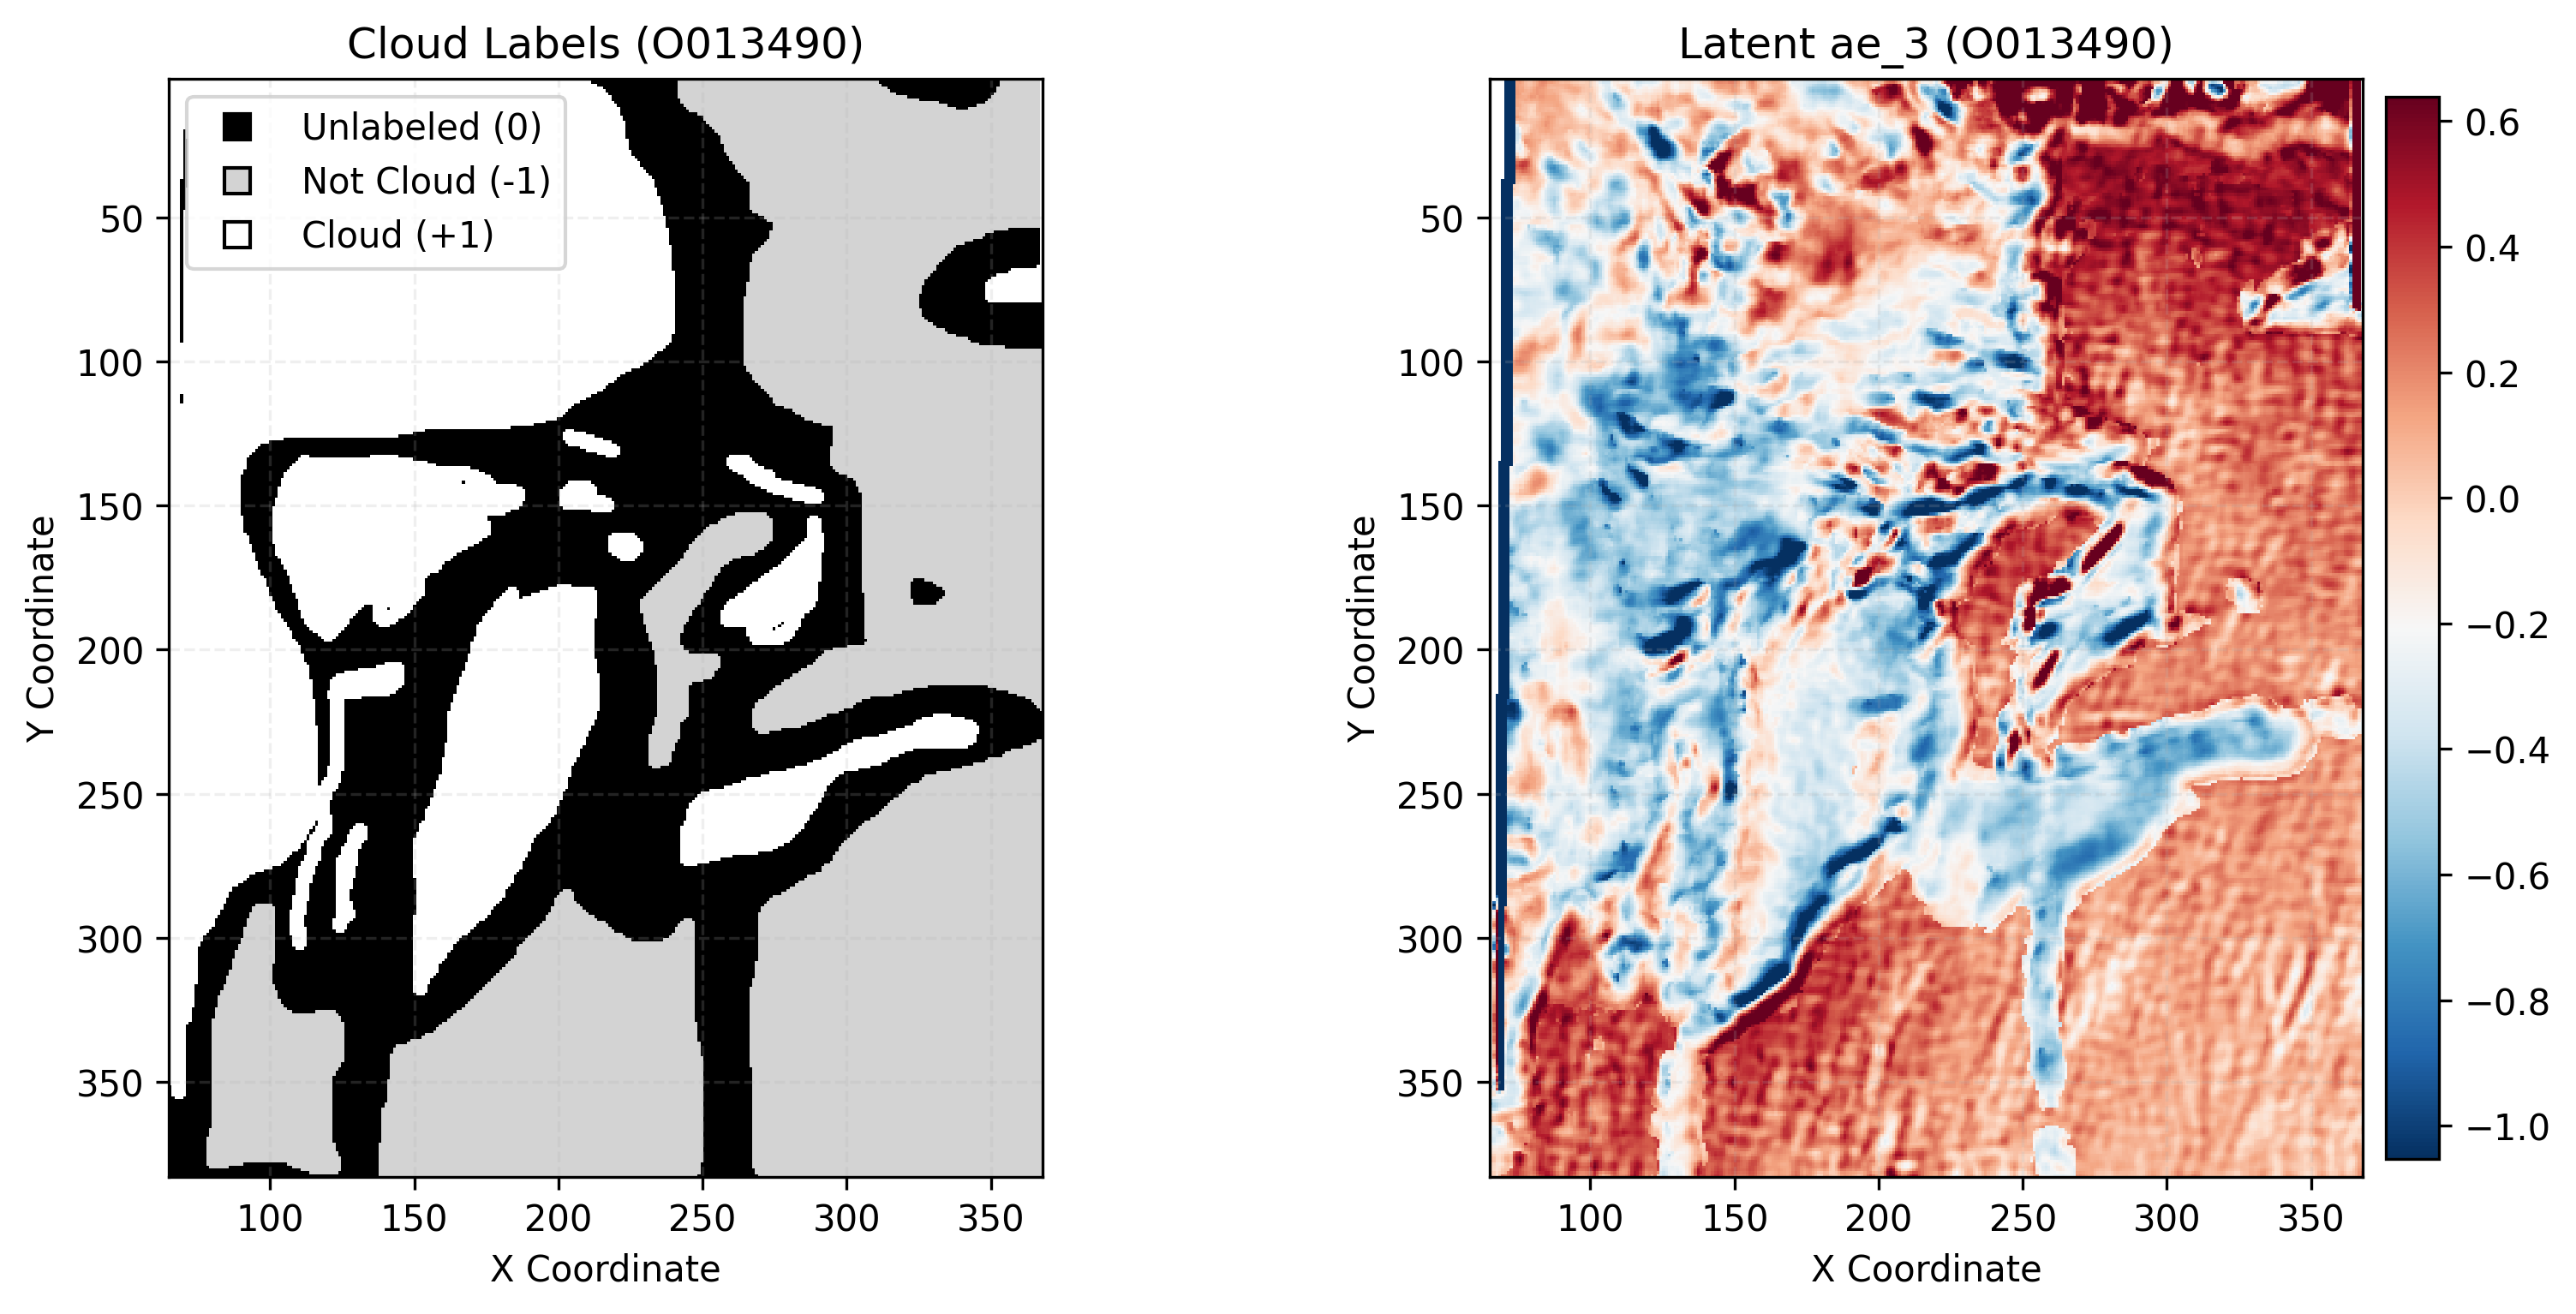
\includegraphics[width=0.7\linewidth]{../figs/O013490_latent_ae_3.png}
    \caption{Embedding visualization (4th embedding feature) of the final autoencoder}
    \label{fig:embedding_visualization}
\end{figure}

From the above results, we can conclude that the transfer learning pipeline with the selected autoencoder architecture is effective in learning meaningful cloud representations from limited labeled data. The learned representations can be further used for downstream cloud prediction tasks, which will be described in the next section.

However, there are still some limitations to our current approach. First, the current evaluation metrics focus on reconstruction quality, which may not directly reflect the usefulness of the learned representations for downstream tasks. Second, due the limitation of computational resources, we only experimented with a limited set of architectures and hyperparameters. And experiments can be repeated with multiple random seeds to increase the robustness of the results. Future work can focus on filling these two gaps.



\section{Modeling}


\subsection{Models}

With newly engineered features and latent factors from the autoencoder, we evaluated four binary classifiers: logistic regression, support vector machine (SVM), extreme gradient boosting (XGBoost), and Light Gradient Boosting Machine (LightGBM). Logistic regression served as a baseline, being a classical method for binary classification. SVM with a Gaussian kernel introduces non-linear relationships.
XGBoost does not assume linearity distribution of the data like logistic regression and linear SVM. Also, few assumptions are required for XGBoost, as scaling and normality are not required. Similar, but even faster, LightGBM offers high accuracy and excels at large datasets. LightGBM’s computational efficiency comes from its reliance on its histogram-based decision tree learning algorithm. 


\subsubsection{Logistic Regression}

We used the image-based split for logistic regression and SVM because these simpler models rely on feature quality than on larger sample size. Moreover, it minimized spatial data leakage from neighboring pixels, leading to a more reliable evaluation of generalization. 

Based on our EDA and feature construction, strong multicollinearity existed among features, which can make distance-based model unstable and vulnerable. To mitigate this, we applied a strict feature selection pipeline: removing near-zero variance features, filtering highly correlated features (threshold 0.95), and sequentially selecting features via mutual information, random forest importance, and VIF. This reduced the original 112 features to 6 key features, including original expert features, engineered spatial features, and one latent factor (ae3) from the autoencoder.

Despite this, the baseline logistic regression model exhibited overfitting, with high training performance but low validation recall, indicating difficulty in capturing complex patterns and identifying cloud pixels. After tuning (elastic net, class weights, and threshold) to optimize F1 score, validation performance improved substantially. However, performance dropped again on the test set, suggesting remaining overfitting or distribution shift.

In terms of interpretability, standardizing features in preprocessing stage allows for direct comparison. As it is shown in Figure ~\ref{lr-coef}, SD and NDAI had significant positive effects, consistent with domain knowledge, while some correlation-based features show less stable or counterintuitive effects, likely due to multicollinearity. Also, the latent factor \textbf{ae3} was not strongly correlated with other features but showed large-magnitude coefficient, suggesting it successfully captured unique patterns relevant for cloud detection.

\subsubsection{Support Vector Machine (RBF Kernel)}


Jumping from a linear model to a non-linear model, we trained an SVM with a Gaussian kernel to capture non-linear relationships missed before, while keeping a relatively simple model structure. We used the same feature set as the logistic regression model and tuned C, gamma, and class weight. The best SVM achieved a validation recall of 0.46, F1-score of 0.61, and AUC of 0.95. 

On the test set, the SVM demonstrated small improvement over logistic regression, with accuracy of 0.80, recall of 0.36, precision of 0.87, F1-score of 0.51, and AUC of 0.85. This suggested better generalization, likely due to its ability to capture non-linear relationships. Unfortunately, the gaussian kernel SVM had improved ability to identify non-cloud units but still performed poorly on cloud units.

Although SVM was less interpretable, especially with non-linear kernels, we used permutation importance (measured by F1 decrease) for interpretation. The results were consistent with logistic regression, with SD, ae3, and NDAI being the most influential features in Figure ~\ref{svm-importance}. 

In contrast, several correlation-based features (e.g., CORR, CORR\_13\_max) showed near-zero or negative importance, suggesting redundancy or noise due to multicollinearity. Permuting these features slightly improved performance, indicating they may hinder generalization.

\begin{figure}[htbp]
    \centering
    \begin{subfigure}[t]{0.48\textwidth}
        \centering
        
\includegraphics[width=\textwidth]{../figs/lr_coefficients.png}
        \caption{Logistic regression coefficients}
        \label{lr-coef}
    \end{subfigure}
    \hfill
    \begin{subfigure}[t]{0.48\textwidth}
        \centering
        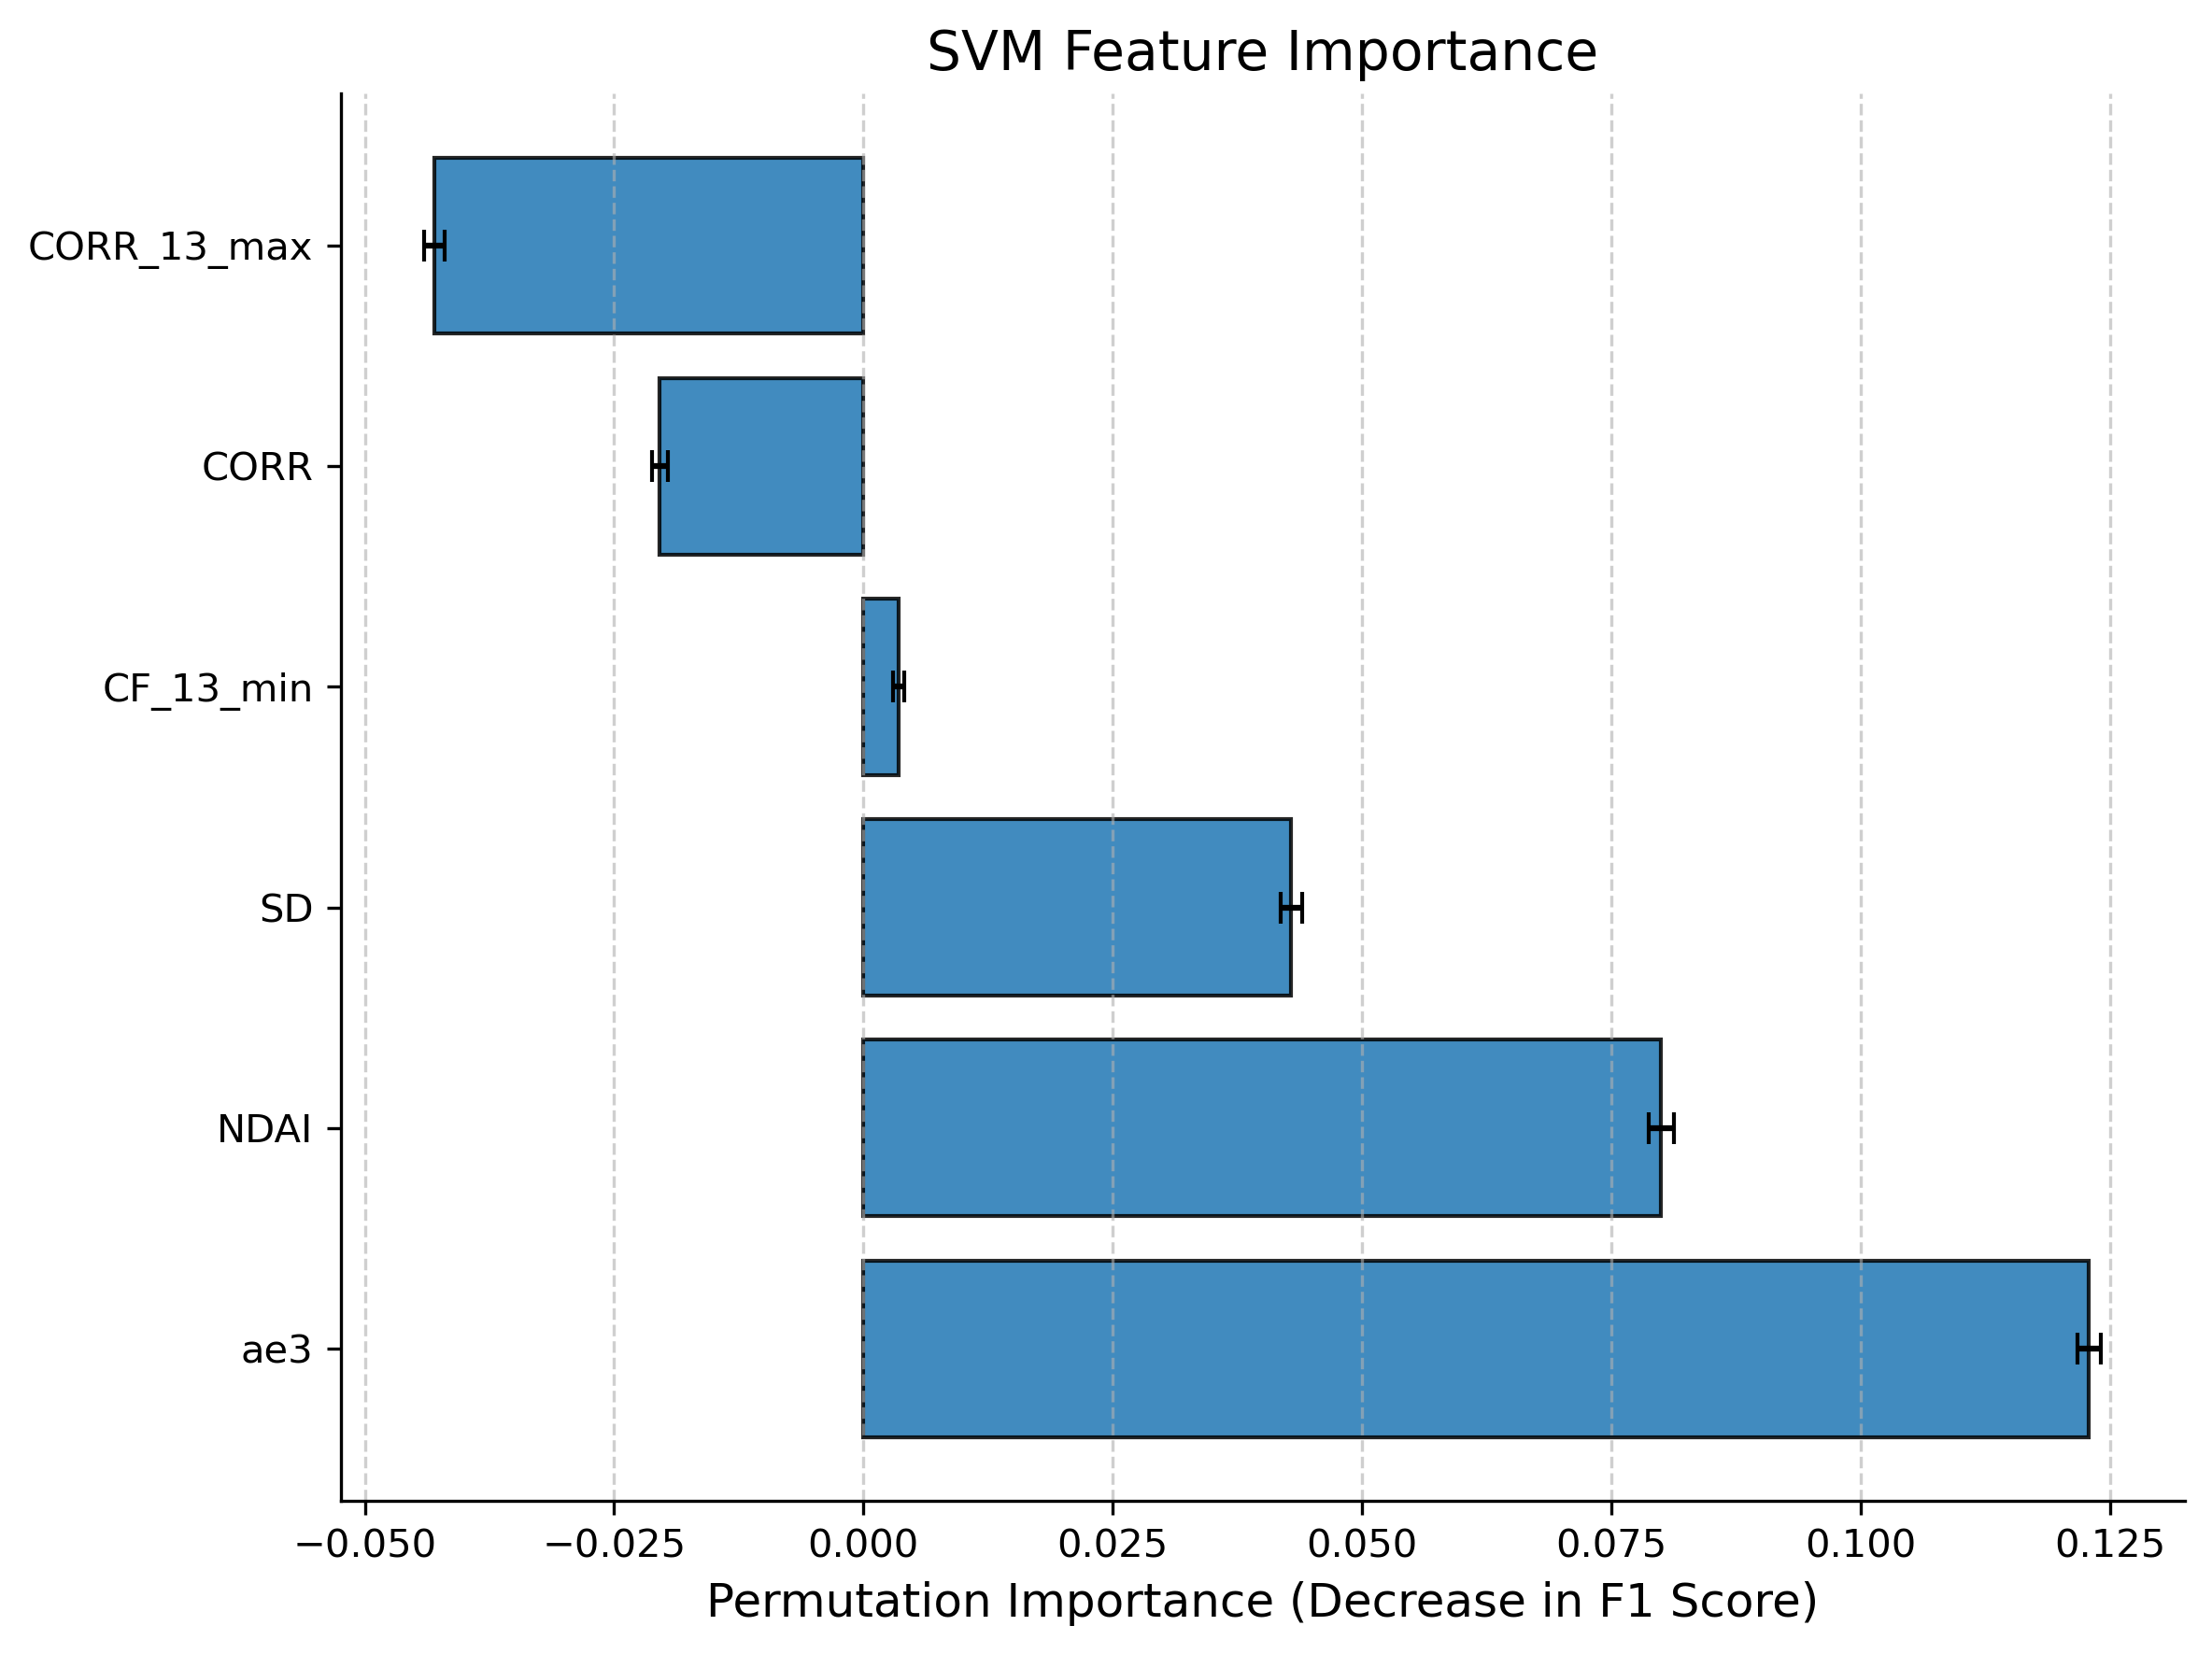
\includegraphics[width=\textwidth]{../figs/svm_feature_importance.png}
        \caption{SVM permutation importance} 
        \label{svm-importance}
    \end{subfigure}
    
    \caption{Feature interpretation for logistic regression and SVM.}
\end{figure}

\subsubsection{XGBoost}

XGBoost shows a strong ability in handling outliers and multicollinearity with high success. All 112 features (those provided by the original images, newly engineered features, and autoencoder-derived representations) were included as an exploratory step of this classifier. XGBoost is very effective at feature selection, because it automatically ranks features by importance during training. The top 25 features were taken and features which had correlation greater than 0.9 were removed, resulting in 16 features. The resulting model had an ROC AUC score of 0.95. 

The main issue that arose with XGBoost was its tendency to underrepresent clouds. While XGBoost had high precision for evaluating clouds, it also had very poor recall resulting in a high number of false negatives. A common reason for this type of result is the impact of imbalance data. While the training image had balanced classification, validation and test images did not. However, even following cross validation and tuning for weight XGBoost still had poor recall for cloud points. In researching patterns that can throw off XGBoost, a significant limitation of tree-based models in general is that they cannot extrapolate trends outside the range of the training data. Because this implementation only relied on one image at a time to train on, the model was unable to tune for different cloud patterns. As we saw in the EDA, occurrences like movement in clouds result in different radiance patterns. Our engineered features are still based on these attributes and these differences are still very relevant.



\subsubsection{LightGBM}


Due to the limitation we found during XGBoost training, to further improve the robustness of our models to spatial variability, we extended the training setup to incorporate multiple images with quadrant-based splits.

LightGBM is a model designed to enhance the performance of decision trees through gradient boosting. A key characteristic of this approach is that it leverages both training and validation data during the learning process, iteratively minimizing the difference between predicted and actual values on the validation set. While this method can increase computational cost as the dataset grows, LightGBM mitigates this issue by employing various optimization techniques to accelerate training.

For hyperparameter tuning, we applied cross-validation based on four quadrants as discussed in Section~\ref{sec: quadrant-based} . The number of leaves was tested over the values [15, 31, 63], and the learning rate over [0.05, 0.1, 0.15]. The optimal configuration was found to be 15 leaves and a learning rate of 0.15. 

During this process, we observed that the LightGBM model tended to perform worse in terms of accuracy when more features were included, both in the train/test split and during cross-validation. After multiple experiments, we decided to remove all features related to the variables AF, BF, CF, DF, and AN. This led to an improvement in accuracy from 98.2\% to 98.6\%. 
% Notably, this feature selection step significantly benefited only the LightGBM model, which is why it was applied exclusively to it.

% The test results are presented below. An accuracy of 98.6\% represents the best performance among the three models.

With this parameter setup, the resulting confusion matrix is as follows:
\begin{table}[h!]
\centering

\label{tab:lightgbm_confusion_matrix}
\begin{tabular}{c|cc}
\hline
\textbf{True} $\backslash$ \textbf{Predicted} & \textbf{0} & \textbf{1} \\
\hline
\textbf{0} & 41,755 & 1,075 \\
\textbf{1} & 67    & 39,186 \\
\hline
\end{tabular}
\caption{LightGBM confusion matrix in test image.}
\end{table}
\subsubsection{Comparison}

Overall, we decided to go with LightGBM over logistic regression, SVM, and XGBoost because of its ability to perform efficiently. As shown in Table~\ref{tab:performance_comparison}, LightGBM achieved the best results across all evaluation metrics, including an F1 score of 0.98 on the test set, indicating a well-balanced trade-off between precision and recall in our imbalance dataset.


Compared with logistic regression and SVM, LightGBM can capture complex nonlinear patterns without manual feature selection, thorough hyperparameter tuning and careful threshold choosing. In addition, it demonstrated stable behavior than XGBoost, particularly in avoiding the high false negative rate observed in that model.

Despite its strong performance, LightGBM can be prone to overfitting due to its leaf-wise tree growth strategy. To mitigate this risk, we further examined model stability under noise and across different preprocessing judgment calls in Section~\ref{sec:stability-check}, ensuring that the learned patterns are robust and generalizable.

\begin{table}[H]
\centering
\begin{tabular}{llccccc}
\hline
Model & Dataset & Accuracy & Recall & Precision & F1 Score & AUC \\
\hline
\multirow{2}{*}{Logistic Regression}
& Validation & 0.80 & 0.52 & 0.93 & 0.66 & 0.94 \\
& Test       & 0.78 & 0.40 & 0.71 & 0.53 & 0.74 \\
\hline
\multirow{2}{*}{SVM (RBF)}
& Validation & 0.78 & 0.46 & 0.92 & 0.61 & 0.95 \\
& Test       & 0.80 & 0.36 & 0.87 & 0.51 & 0.85 \\
\hline
\multirow{2}{*}{XGBoost} 
& Validation & 0.79 & 0.79 & 0.82 & 0.77 & 0.95 \\
& Test       & 0.80 & 0.80 & 0.84 & 0.77 & 0.98 \\
\hline
\multirow{1}{*}{LightGBM} 
& Validation & 0.97 & 0.97 & 0.97 & 0.93 & 0.92 \\
& Test       & 0.98 & 0.98 & 0.98 & 0.98 & 0.93 \\
\hline
\end{tabular}
\caption{Performance comparison between multiple classifiers.}
\label{tab:performance_comparison}
\end{table}

\subsection{Post-hoc Evaluation}

As a post-hoc EDA step, we compare the predictions from the LightGBM models with the ground-truth expert labels. While the overall high accuracy indicates strong agreement with the expert labels, some discrepancies remain—primarily at the image boundaries and the central regions of the images.


\begin{figure}[H]
    \centering
    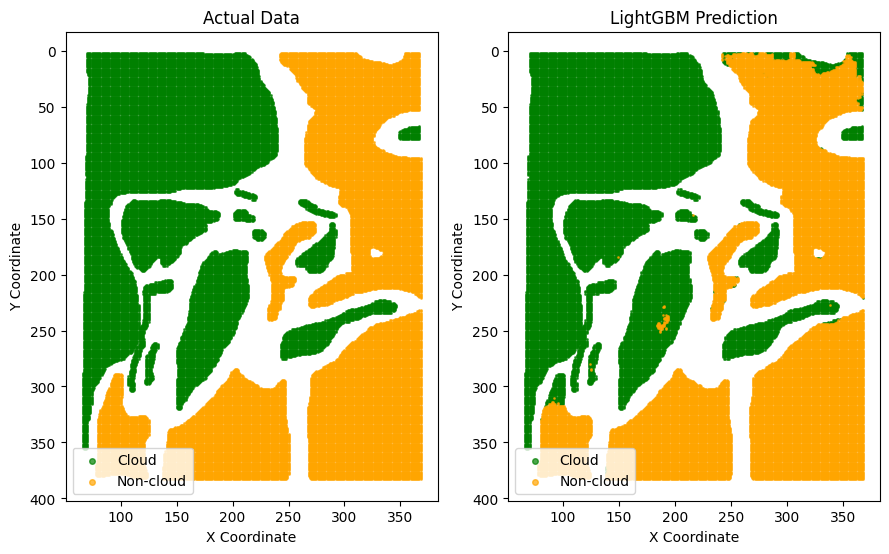
\includegraphics[width=0.75\linewidth]{../figs/Post-hoc.png}
    \caption{Comparison of expert labels and model predictions}
    \label{fig:Post-hoc}
\end{figure}

Prediction errors near the image boundaries can be explained by the limited availability of contextual information, as it is not possible to fully capture all neighboring pixels at the edges. In particular, when patches are constructed (e.g., for autoencoder-based features), missing values at the borders are often handled by flipping the image and filling in the gaps. However, this approximation introduces artifacts, and the resulting errors from this process are non-negligible.

Prediction errors in the central region of the image can be linked to the key feature SD\_mean\_13. Analyzing its distribution on the test data shows that the center area is highlighted similarly to cloud-free regions, which leads to misclassification. In other parts of the image, however, SD\_mean\_13 aligns well with the expert labels, indicating that it is generally a strong predictive feature, though not sufficient on its own to capture all patterns.

Interestingly, performance in the central region improves when the magnitude of this feature is reduced. This suggests that scaling down feature values helps achieve a better balance among variables, allowing the model to rely more effectively on multiple features rather than being overly influenced by a single one.

\begin{figure}[H]
    \centering
    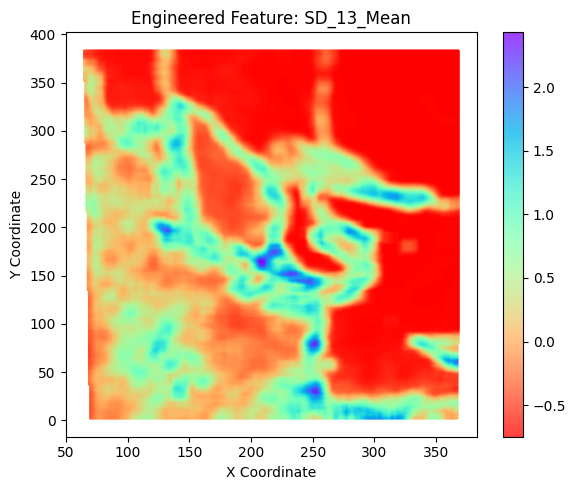
\includegraphics[width=0.4\linewidth]{../figs/sd13.png}
    \caption{Distribution of the engineered feature SD\_mean\_13}
    \label{fig:sd13}
\end{figure}

\subsection{Stability Check}\label{sec:stability-check}

\subsubsection{Stability to Data Perturbations}

To evaluate the stability of our analysis, we first introduced perturbations in our original training data and evaluated across the entire data science pipeline. One way to perturb image data is to introduce statistical noise to the existing features. One common example of noise is Gaussian noise. Gaussian noise impacts all pixels in the perturbed image(s) by introducing low-level variations (following a normal distribution) to features. 
Filepaths to the training images are loaded through our perturbation function (see \textit{stability.py} and \textit{stability.ipynb}) and new NPZ files are stored. 
From there, we are able to train our LightGBM model pipeline using autoencodings and engineered features. Despite these perturbations in the data, the most important features remained consistent. The exact order after perturbations did not match; however, the inclusion alludes to the stability of our model. The associated confusion matrix aligns closely with the baseline model's performance on the original dataset.  


\begin{figure}[htbp]
    \centering

    % Left: Original
    \begin{subfigure}{0.45\textwidth}
        \centering
        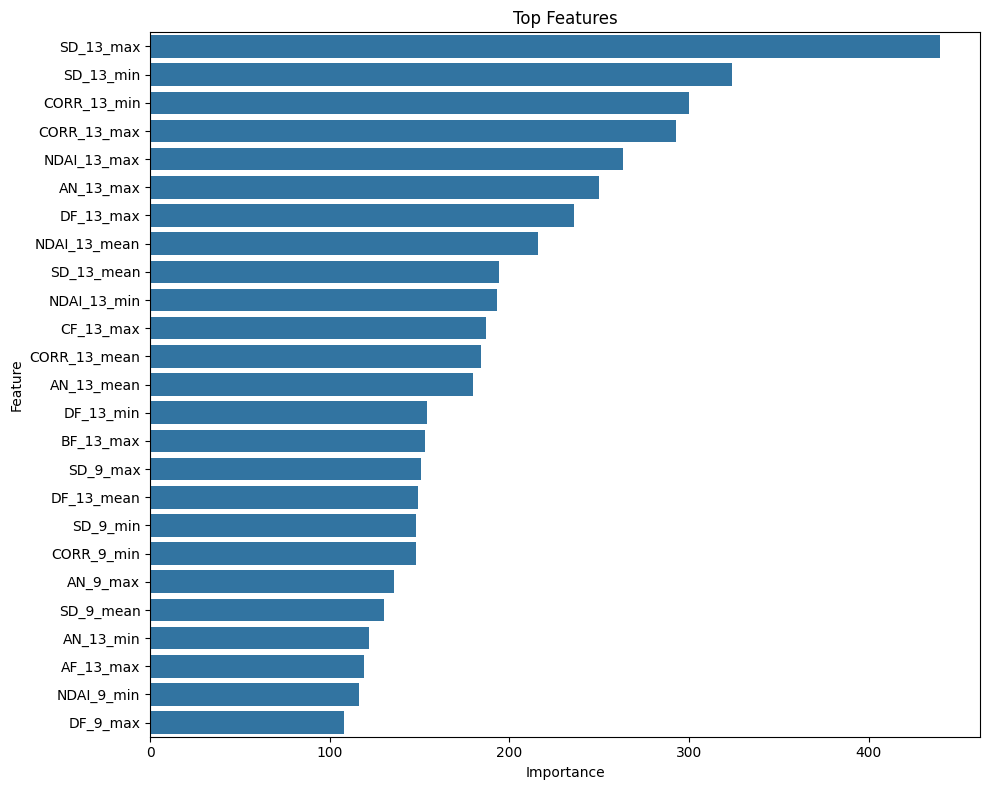
\includegraphics[width=\linewidth]{../figs/og_feature_importance.png}
        \caption{Original}
        \label{fig:original}
    \end{subfigure}
    \hfill
    % Right: Perturbed
    \begin{subfigure}{0.45\textwidth}
        \centering
        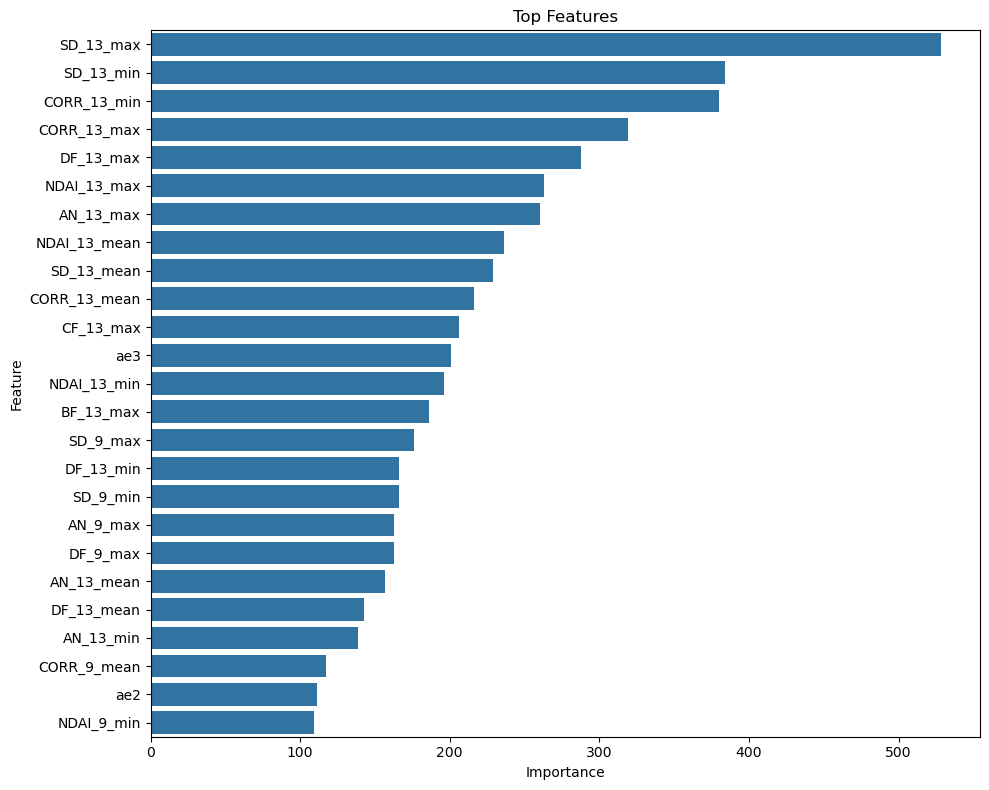
\includegraphics[width=\linewidth]{../figs/stability_feature_importance.png}
        \caption{Perturbed}
        \label{fig:stability}
    \end{subfigure}
    
    \caption{Comparison of feature importance between the original and Gaussian noise–perturbed datasets. While minor changes in feature ranking are observed, the key features remain consistent, indicating the stability of the model under perturbations.}
    \label{fig:feature_importance_comparison}
\end{figure}


\subsubsection{Stability to Data Cleaning and Preprocessing Judgment Calls}


To evaluate the stability of our analysis to data cleaning and preprocessing judgment calls, we consider different combinations of data cleaning and preprocessing steps. As mentioned in the EDA section, we have identified some potential data quality issues, such as outliers. Two preprocessing judgement calls are considered in this analysis, including $3\sigma$ outlier removal and Z-score standardization. We retrain and evaluate the performance of our model under different combinations of these preprocessing steps and compare the results.

\newlength{\stabilityH}
\setlength{\stabilityH}{0.33\textheight}

\begin{figure}[htbp]
    \centering
    \begin{minipage}[c][\stabilityH][c]{0.48\linewidth}
        \centering
        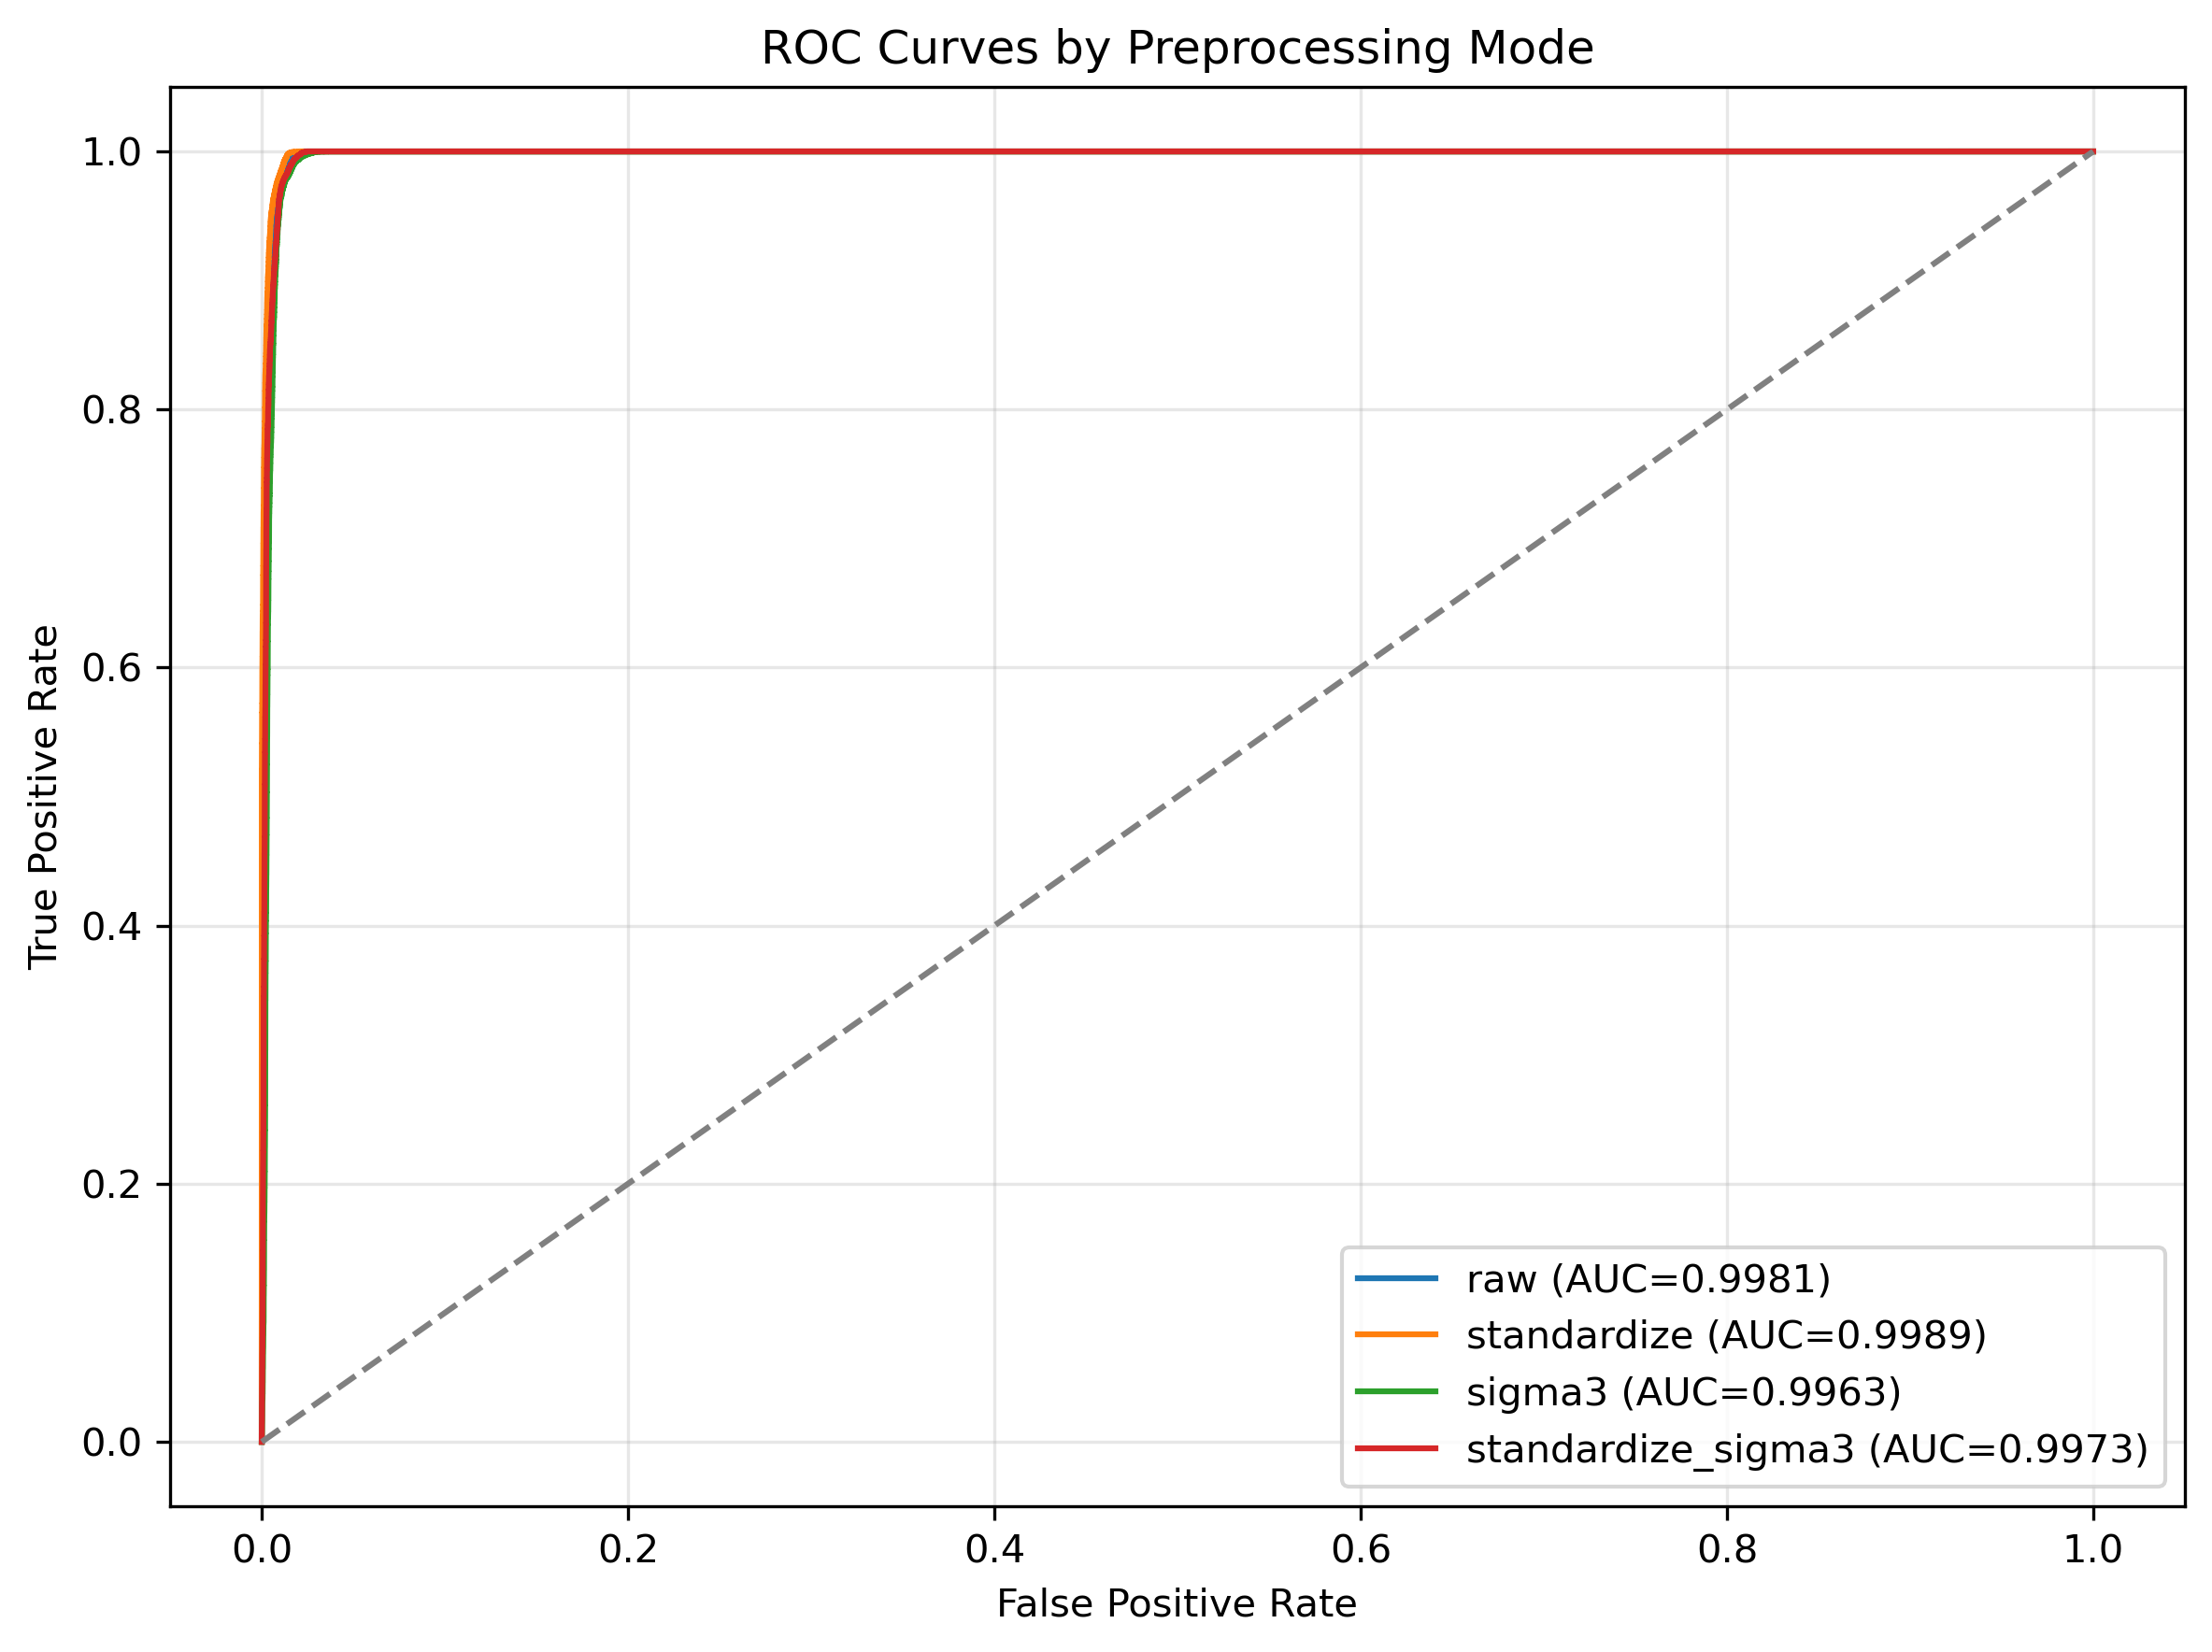
\includegraphics[width=\linewidth,height=\stabilityH,keepaspectratio]{../figs/stability_judgement_call_roc.png}
    \end{minipage}\hfill
    \begin{minipage}[c][\stabilityH][c]{0.50\linewidth}
        \centering
        \footnotesize
        \renewcommand{\arraystretch}{1.18}
        \setlength{\tabcolsep}{4pt}
        \begin{tabular}{@{}lccc@{}}
        \toprule
        Judgement call & F1 $\uparrow$ & AUC $\uparrow$ & CV best score $\uparrow$ \\
        \midrule
        Raw                  & 0.987124          & 0.998074          & 0.927557 \\
        Standardize          & \textbf{0.988342} & \textbf{0.998884} & 0.927331 \\
        $3\sigma$ filter     & 0.981893          & 0.996296          & \textbf{0.935587} \\
        Std. + $3\sigma$ filter & 0.983888       & 0.997350          & 0.932361 \\
        \bottomrule
        \end{tabular}
    \end{minipage}
    \caption{Stability of model performance under different preprocessing judgement calls}
    \label{fig:preprocessing_stability}
\end{figure}



The results are summarized in Figure~\ref{fig:preprocessing_stability}. We observe that there are only minor variations in the ROC curve under different combinations of preprocessing steps, which indicates that the model performance is relatively stable to these judgment calls. The AUC values are also similar across different combinations, which further supports the stability of our model.


\subsection{Reality Check}

In this section, we performed a reality check to assess whether our best classifier behaves reasonably beyond random guessing. Since our dataset contains only three labeled images, this reality check focused on the unlabeled images. By comparing the predictions with domain knowledge, we could qualitatively evaluate whether the model outputs are plausible. 

For instance, if the classifier predicts that an unlabeled image consists of nearly 99\% cloud pixels, this would raise concerns about model validity, as such extreme distributions are unlikely in practice. For the reality check, we randomly selected three unlabeled images [Image O002539, Image O002772 and Image O003005], applied the same feature engineering pipeline (including the newly constructed spectral features and autoencoder representations), and used the best classifier to generate pixel-level cloud probabilities.

\subsubsection{Spatial Visualization}

We first presented a summary of the predicted cloud probabilities for the three unlabeled images. Table~\ref{tab:unlabeled_summary} reports the number of pixels, mean, median, standard deviation, and predicted cloud rate for each image. 

A key observation was that the mean predicted probability is very close to the predicted cloud rate for each image. This suggested that most predicted probabilities were concentrated near the extremes (0 or 1), indicating that the model outputs are highly polarized rather than diffuse.

\begin{table}[H]
\centering
\footnotesize 

\setlength{\tabcolsep}{4pt}   
\renewcommand{\arraystretch}{1.1} 
\caption{Summary statistics of predicted cloud probabilities by image}
\label{tab:unlabeled_summary}
\begin{tabular}{lcccccc}
\toprule
Image ID & Pixels & Mean & Median & Std & Cloud Rate \\
\midrule
O002539 & 115,378 & 0.883 & 1.000 & 0.302 & 0.885 \\
O002772 & 115,668 & 0.081 & 0.000 & 0.261 & 0.081 \\
O003005 & 115,923 & 0.753 & 1.000 & 0.409 & 0.756 \\
\bottomrule
\end{tabular}
\end{table}


The spatial visualization in Figure~\ref{fig:prediction_panel_unlabeled} further supported this observation. The predicted probability maps closely resembled the corresponding binary label maps, indicating that most predictions lie near the decision threshold. This consistency suggested that the classifier produces stable spatial patterns, rather than noisy or fragmented predictions.

\begin{figure}[H]
\centering
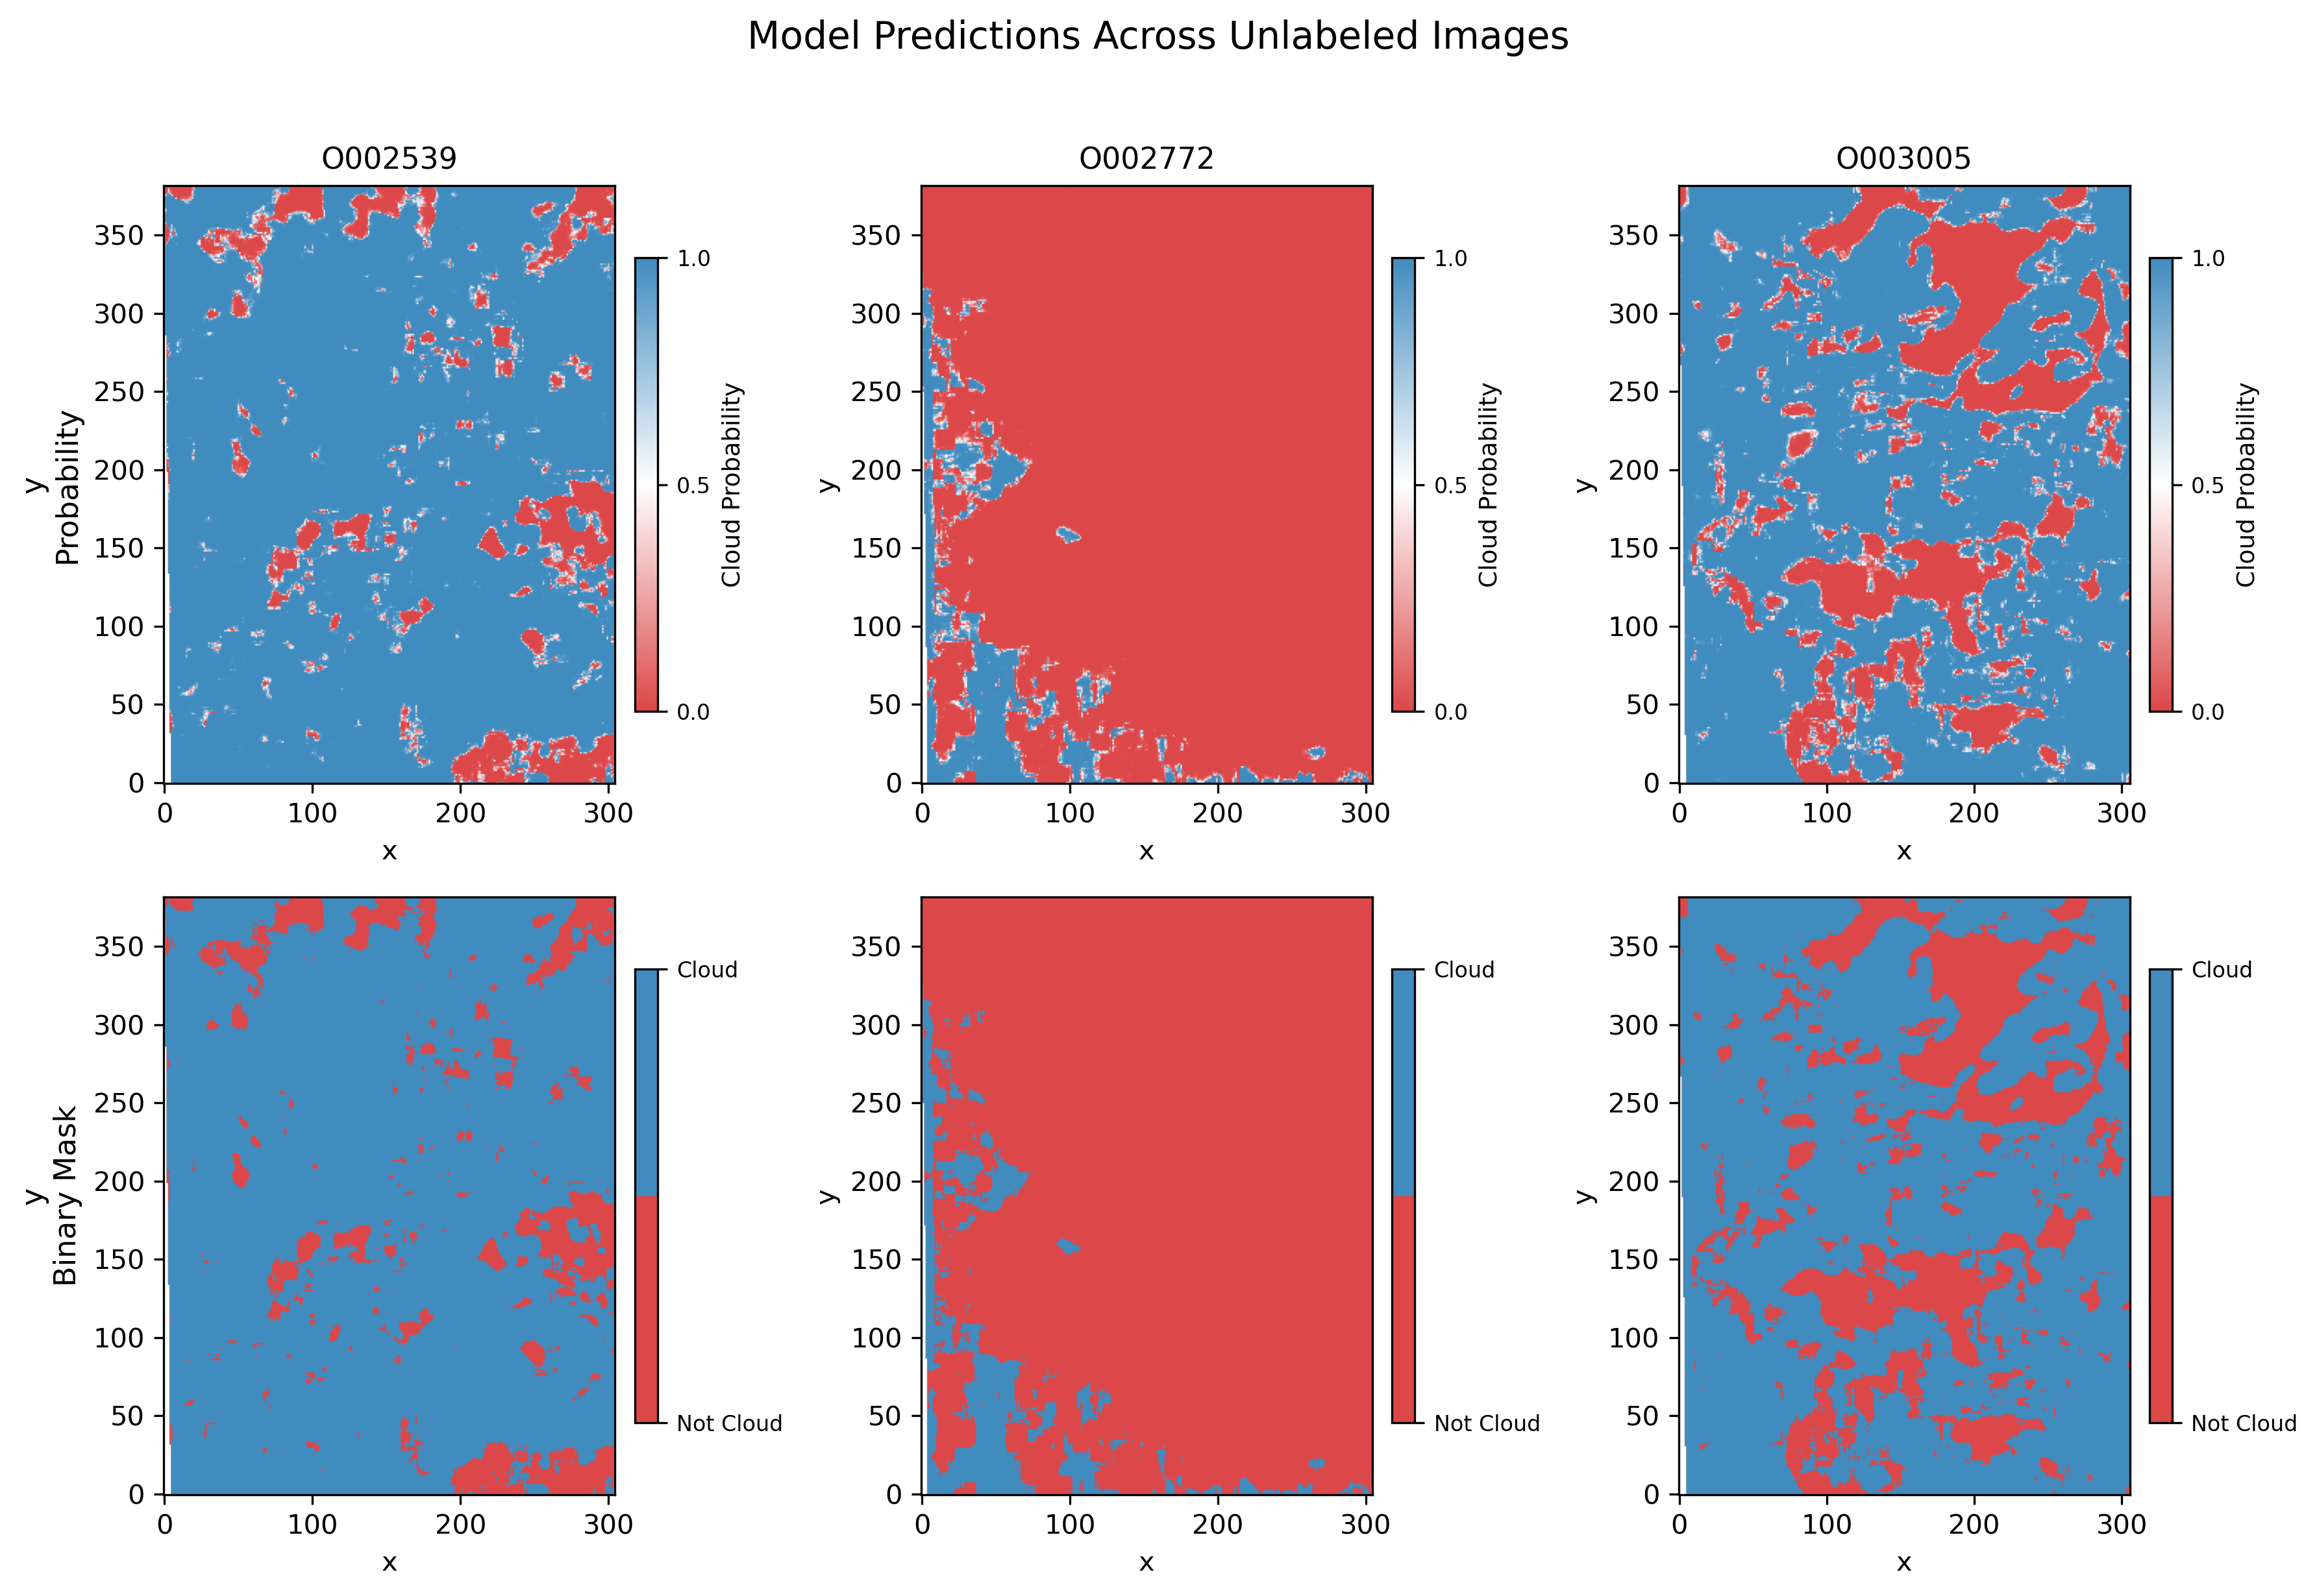
\includegraphics[width=0.8\textwidth]{../figs/prediction_panel_unlabeled.png}
\caption{Spatial visualization of predicted cloud probabilities and labels for three unlabeled images. The blue represents the cloud pixels while the red represents the non-cloud ones. The first row shows the predicted cloud probabilities, and the second row shows the predicted cloud labels.}
\label{fig:prediction_panel_unlabeled}
\end{figure}

\subsubsection{Predicted Cloud Probability Distribution}


The predicted cloud probability distribution figure again validated our assumption that the predicted cloud probabilities are very close to either 0 or 1, since the predicted cloud probabilities are highly skewed towards 0 and 1. This indicated that the model produces highly confident predictions rather than uncertain ones. Such behavior suggested that the decision boundary is sharp, insensitive to threshold. However, since we evaluated on the unlabelled data, this high level of confidence led us to caution about overfitting or sensitvity to training data distribution.

\begin{figure}[htbp]
\centering
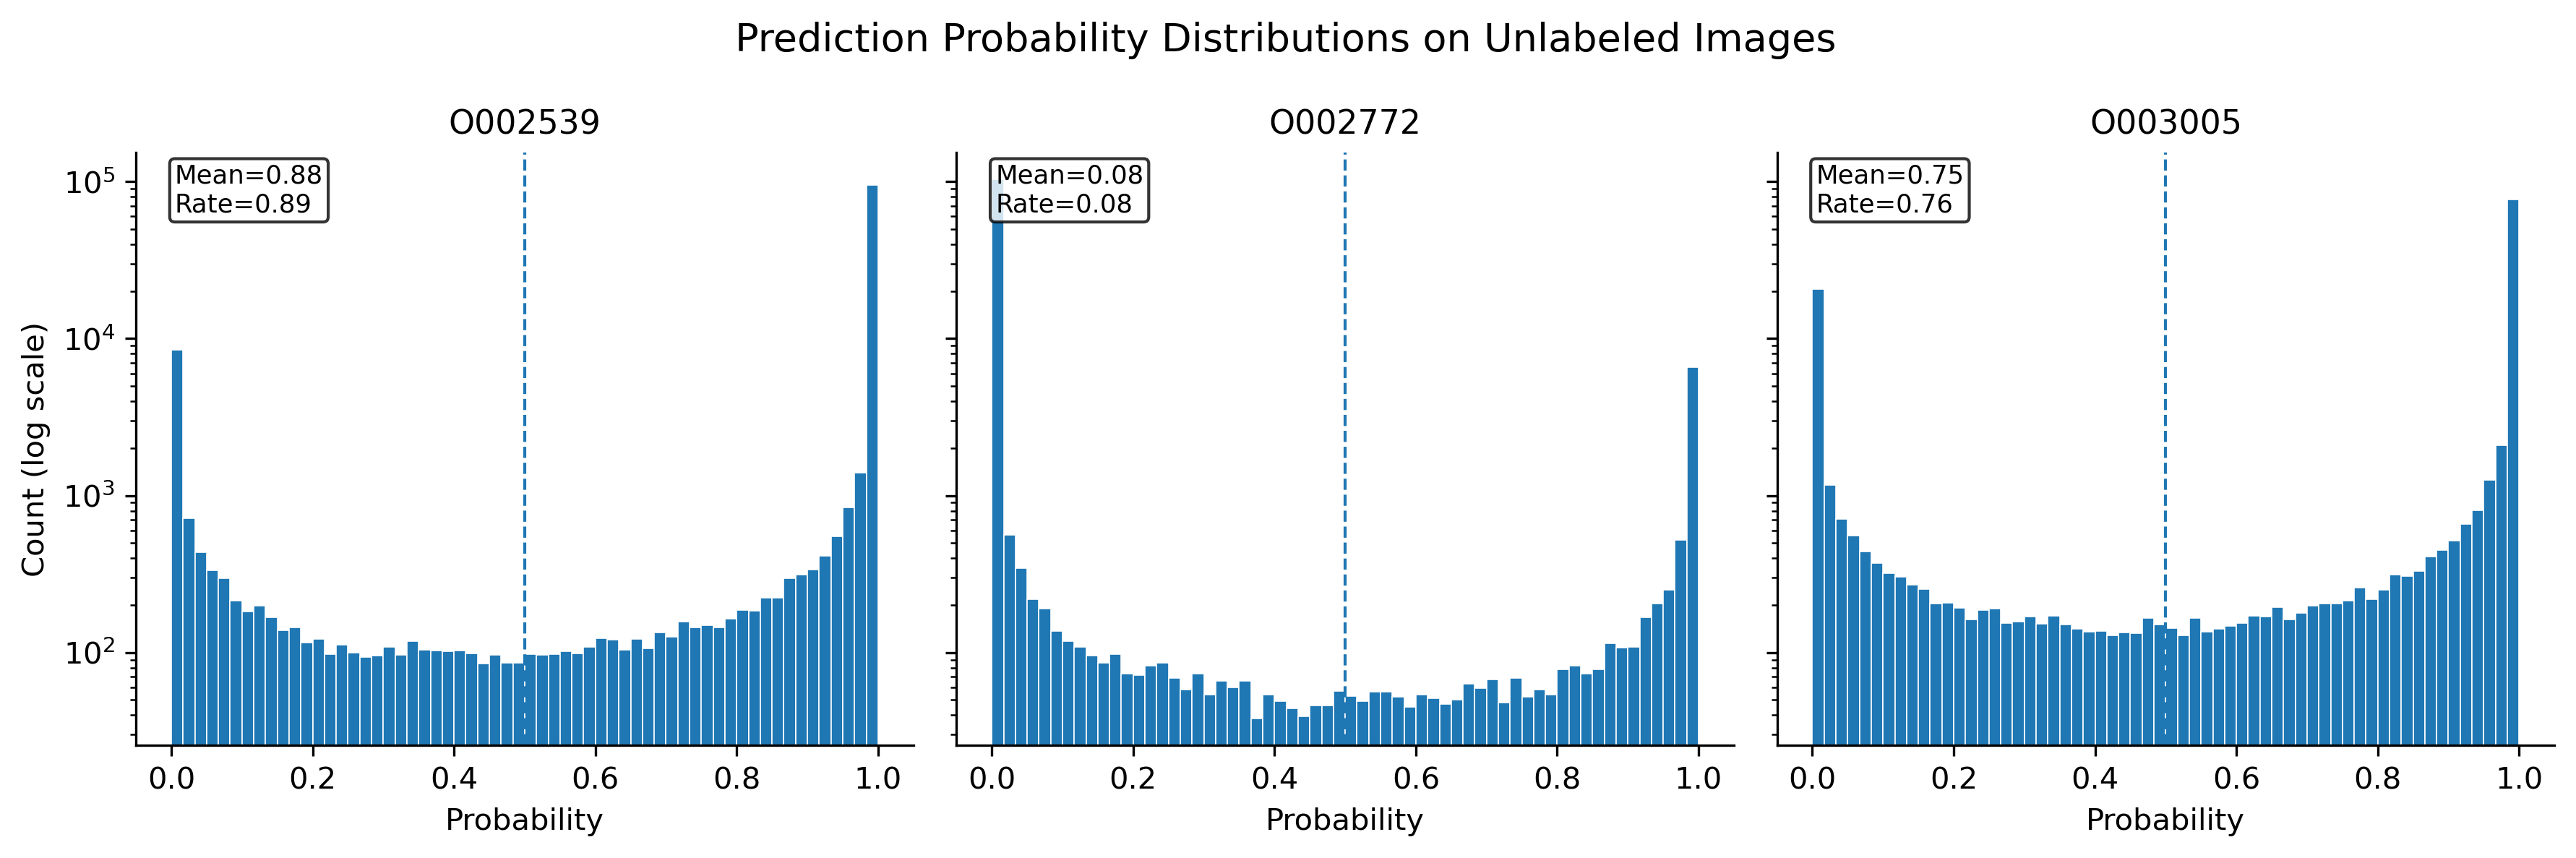
\includegraphics[width=0.95\textwidth]{../figs/probability_histograms_unlabeled.png}
\caption{Predicted cloud probability distribution for three unlabeled images. The y-axis is shown on a logarithmic scale to better visualize the distribution of probabilities near 0 and 1.}
\end{figure}


\subsubsection{Feature-level Reality Check}


As an additional validation, we examined the distributions of three expert-designed features: SD, CORR, and NDAI. We plot boxplots of these features grouped by predicted cloud labels for the three unlabeled images.

Encouragingly, the observed patterns were largely consistent with domain knowledge \cite{shi_daytime_2008} and our earlier exploratory data analysis. In particular, SD tended to be higher for predicted cloud pixels, reflecting greater variability in radiance values. Similarly, NDAI was higher for cloud pixels, aligning with its role in capturing angular radiance differences.

In contrast, CORR showed weaker separation between predicted cloud and non-cloud pixels. This may be explained by the presence of low-altitude clouds, which exhibit radiance patterns more similar to the clear conditions, reducing the discriminative power of this feature.


\begin{figure}[htbp]
\centering
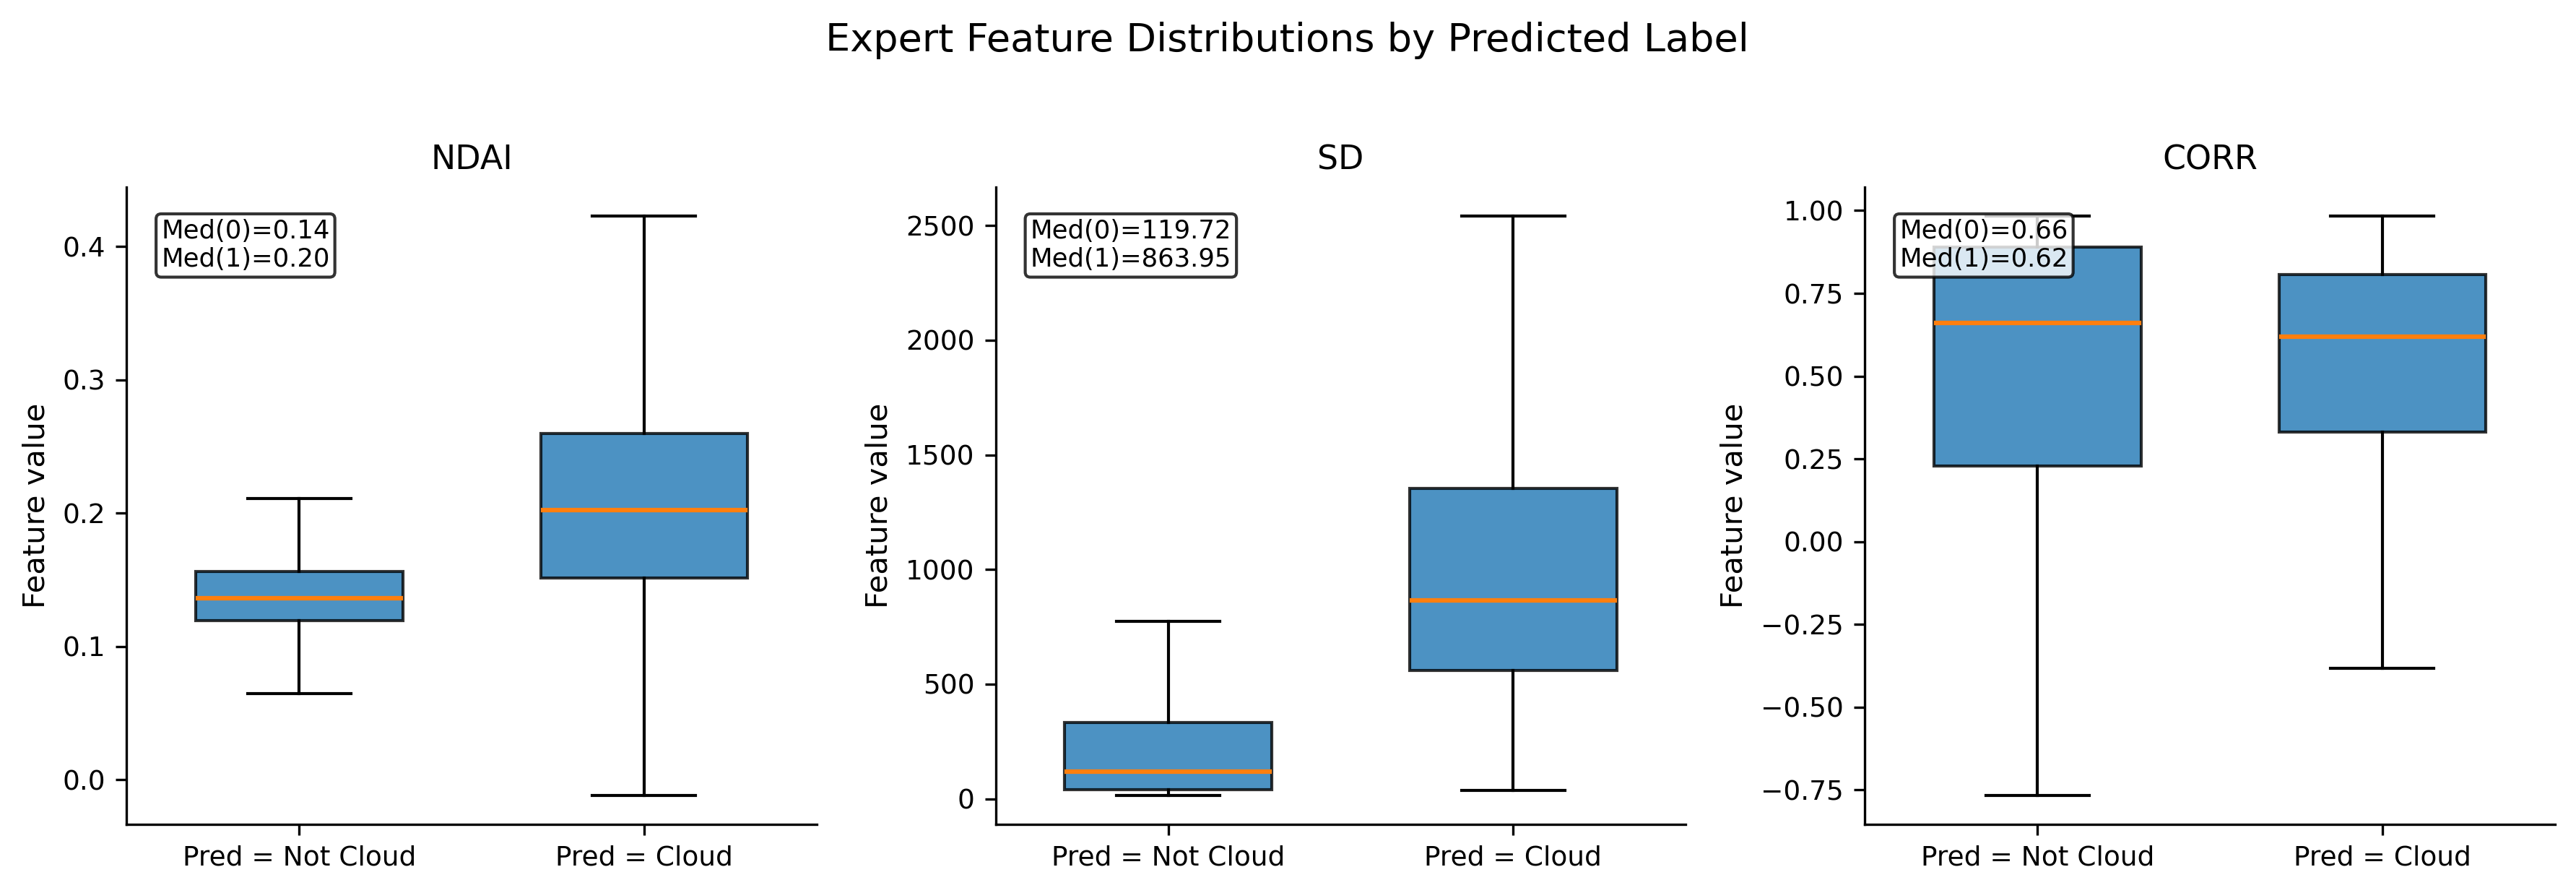
\includegraphics[width=0.95\textwidth]{../figs/feature_boxplots_unlabeled.png}
\caption{Boxplots of three expert features by predicted cloud label.}

\end{figure}


\paragraph{Summary.}
Overall, the reality check suggested that the model produces spatially coherent and highly confident predictions on unlabeled images. The agreement between probability maps and predicted labels, along with the polarized probability distributions, indicated that the classifier had learned a sharp decision boundary.

Moreover, the feature-level analysis showed that the predicted cloud labels were largely consistent with known physical patterns of key features such as SD and NDAI, providing additional support for the plausibility of the predictions. 

However, since these assessments were based on unlabeled data, they could not provide definitive evidence of predictive accuracy. The high confidence of the model also raised potential concerns about overfitting or sensitivity to the training distribution. Therefore, while the reality check increased our confidence in the model’s behavior, the results should be interpreted with caution.

\section{Conclusions}

Overall, we achieved accurate and reliable cloud detection in daylight Arctic conditions by combining domain-informed feature engineering with models capable of capturing complex patterns. 

Our exploratory data analysis showed that raw MISR angular radiances are strongly correlated,  indicating redundancy in the feature space and the need for feature engineering to distinguish between cloud and non-cloud pixels.

A preliminary CART analysis showed that the original features, especially SD and CORR, are highly informative. Motivated by spatial patterns observed in EDA, we further expanded the feature set using neighborhood-based statistics to boost our subsequent prediction task.

In addition, we incorporated representation learning through an autoencoder with pretraining and fine-tuning, which produced 8-dimensional embeddings. The selected autoencoder architecture is a convolutional autoencoder with 3 layers and 48/96/192 channels with denoising layer, which achieved the lowest reconstruction MSE as 0.118357. The embedding features, such as ae3, capture the patterns at the edge of the cloud, which can be seen from the visualization. The importance of the autoencoder-based features is further supported in the subsequent feature importance analysis.

 With the enriched feature set, we proceeded to train and evaluate a range of classification models. Among all of them, LightGBM achieved the best overall performance, effectively balancing precision and recall, with an AUC of 0.93, recall of 0.98, and F1 score of 0.98. LightGBM successfully captured the underlying nonlinear relationships that simpler models failed to detect. The model demonstrated robustness to data perturbations, where we introduced Gaussian noise to the original features. We also checked the model's stability to data cleaning and preprocessing judgment calls. The results remained robust under different standardization and outlier handling strategies.

It is important to note that there are several limitations in this analysis. Only a small number of labeled images were available, and potential overfitting was suggested by the highly confident predictions. Our reality check further revealed concerns about extremely sharp decision boundaries. Future work should focus on refining the feature selection procedure and modifying model structures to enhance generalizability.


\newpage
\nocite{*}
\bibliography{references}

\newpage
\appendix
\section{Academic honesty}
% Note that this section (and the bibliography) don't count towards the page limit.
\subsection{Statement}
% Please include a joint academic honesty statement here. Do NOT include any of your names.

We, the four members of this group, certify that this report represents our own original work. All analyses, code, visualizations, and written explanations were completed collaboratively by the group members.

We confirm that we have adhered to the academic honesty policies of the course and the university. Any external sources, including research papers, software packages, online materials, or discussions with others, have been properly cited where appropriate. 

Each group member has contributed to the development of the project, including aspects such as data exploration, feature engineering, modeling and interpretation of results, and preparation of the report.
\subsection{LLM Usage}

\subsubsection*{Coding}



AI tools (e.g., ChatGPT, GitHub Copilot) were used only to assist with visualization and minor debugging. All core code was developed and verified by the four of us.


\subsubsection*{Writing}

AI tools (e.g., ChatGPT, GitHub Copilot) were used solely for grammar checking and minor phrasing improvements. All ideas, analysis, and writing were developed and reviewed by the four of us.



\end{document}
